


% Header, overrides base

    % Make sure that the sphinx doc style knows who it inherits from.
    \def\sphinxdocclass{article}

    % Declare the document class
    \documentclass[letterpaper,10pt,english]{/usr/share/sphinx/texinputs/sphinxhowto}

    % Imports
    \usepackage[utf8]{inputenc}
    \DeclareUnicodeCharacter{00A0}{\\nobreakspace}
    \usepackage[T1]{fontenc}
    \usepackage{babel}
    \usepackage{times}
    \usepackage{import}
    \usepackage[Bjarne]{/usr/share/sphinx/texinputs/fncychap}
    \usepackage{longtable}
    \usepackage{/usr/share/sphinx/texinputs/sphinx}
    \usepackage{multirow}

    \usepackage{amsmath}
    \usepackage{amssymb}
    \usepackage{ucs}
    \usepackage{enumerate}

    % Used to make the Input/Output rules follow around the contents.
    \usepackage{needspace}

    % Pygments requirements
    \usepackage{fancyvrb}
    \usepackage{color}
    % ansi colors additions
    \definecolor{darkgreen}{rgb}{.12,.54,.11}
    \definecolor{lightgray}{gray}{.95}
    \definecolor{brown}{rgb}{0.54,0.27,0.07}
    \definecolor{purple}{rgb}{0.5,0.0,0.5}
    \definecolor{darkgray}{gray}{0.25}
    \definecolor{lightred}{rgb}{1.0,0.39,0.28}
    \definecolor{lightgreen}{rgb}{0.48,0.99,0.0}
    \definecolor{lightblue}{rgb}{0.53,0.81,0.92}
    \definecolor{lightpurple}{rgb}{0.87,0.63,0.87}
    \definecolor{lightcyan}{rgb}{0.5,1.0,0.83}

    % Needed to box output/input
    \usepackage{tikz}
        \usetikzlibrary{calc,arrows,shadows}
    \usepackage[framemethod=tikz]{mdframed}

    \usepackage{alltt}

    % Used to load and display graphics
    \usepackage{graphicx}
    \graphicspath{ {figs/} }
    \usepackage[Export]{adjustbox} % To resize

    % used so that images for notebooks which have spaces in the name can still be included
    \usepackage{grffile}


    % For formatting output while also word wrapping.
    \usepackage{listings}
    \lstset{breaklines=true}
    \lstset{basicstyle=\small\ttfamily}
    \def\smaller{\fontsize{9.5pt}{9.5pt}\selectfont}

    %Pygments definitions
    
\makeatletter
\def\PY@reset{\let\PY@it=\relax \let\PY@bf=\relax%
    \let\PY@ul=\relax \let\PY@tc=\relax%
    \let\PY@bc=\relax \let\PY@ff=\relax}
\def\PY@tok#1{\csname PY@tok@#1\endcsname}
\def\PY@toks#1+{\ifx\relax#1\empty\else%
    \PY@tok{#1}\expandafter\PY@toks\fi}
\def\PY@do#1{\PY@bc{\PY@tc{\PY@ul{%
    \PY@it{\PY@bf{\PY@ff{#1}}}}}}}
\def\PY#1#2{\PY@reset\PY@toks#1+\relax+\PY@do{#2}}

\expandafter\def\csname PY@tok@gd\endcsname{\def\PY@tc##1{\textcolor[rgb]{0.63,0.00,0.00}{##1}}}
\expandafter\def\csname PY@tok@gu\endcsname{\let\PY@bf=\textbf\def\PY@tc##1{\textcolor[rgb]{0.50,0.00,0.50}{##1}}}
\expandafter\def\csname PY@tok@gt\endcsname{\def\PY@tc##1{\textcolor[rgb]{0.00,0.27,0.87}{##1}}}
\expandafter\def\csname PY@tok@gs\endcsname{\let\PY@bf=\textbf}
\expandafter\def\csname PY@tok@gr\endcsname{\def\PY@tc##1{\textcolor[rgb]{1.00,0.00,0.00}{##1}}}
\expandafter\def\csname PY@tok@cm\endcsname{\let\PY@it=\textit\def\PY@tc##1{\textcolor[rgb]{0.25,0.50,0.50}{##1}}}
\expandafter\def\csname PY@tok@vg\endcsname{\def\PY@tc##1{\textcolor[rgb]{0.10,0.09,0.49}{##1}}}
\expandafter\def\csname PY@tok@m\endcsname{\def\PY@tc##1{\textcolor[rgb]{0.40,0.40,0.40}{##1}}}
\expandafter\def\csname PY@tok@mh\endcsname{\def\PY@tc##1{\textcolor[rgb]{0.40,0.40,0.40}{##1}}}
\expandafter\def\csname PY@tok@go\endcsname{\def\PY@tc##1{\textcolor[rgb]{0.53,0.53,0.53}{##1}}}
\expandafter\def\csname PY@tok@ge\endcsname{\let\PY@it=\textit}
\expandafter\def\csname PY@tok@vc\endcsname{\def\PY@tc##1{\textcolor[rgb]{0.10,0.09,0.49}{##1}}}
\expandafter\def\csname PY@tok@il\endcsname{\def\PY@tc##1{\textcolor[rgb]{0.40,0.40,0.40}{##1}}}
\expandafter\def\csname PY@tok@cs\endcsname{\let\PY@it=\textit\def\PY@tc##1{\textcolor[rgb]{0.25,0.50,0.50}{##1}}}
\expandafter\def\csname PY@tok@cp\endcsname{\def\PY@tc##1{\textcolor[rgb]{0.74,0.48,0.00}{##1}}}
\expandafter\def\csname PY@tok@gi\endcsname{\def\PY@tc##1{\textcolor[rgb]{0.00,0.63,0.00}{##1}}}
\expandafter\def\csname PY@tok@gh\endcsname{\let\PY@bf=\textbf\def\PY@tc##1{\textcolor[rgb]{0.00,0.00,0.50}{##1}}}
\expandafter\def\csname PY@tok@ni\endcsname{\let\PY@bf=\textbf\def\PY@tc##1{\textcolor[rgb]{0.60,0.60,0.60}{##1}}}
\expandafter\def\csname PY@tok@nl\endcsname{\def\PY@tc##1{\textcolor[rgb]{0.63,0.63,0.00}{##1}}}
\expandafter\def\csname PY@tok@nn\endcsname{\let\PY@bf=\textbf\def\PY@tc##1{\textcolor[rgb]{0.00,0.00,1.00}{##1}}}
\expandafter\def\csname PY@tok@no\endcsname{\def\PY@tc##1{\textcolor[rgb]{0.53,0.00,0.00}{##1}}}
\expandafter\def\csname PY@tok@na\endcsname{\def\PY@tc##1{\textcolor[rgb]{0.49,0.56,0.16}{##1}}}
\expandafter\def\csname PY@tok@nb\endcsname{\def\PY@tc##1{\textcolor[rgb]{0.00,0.50,0.00}{##1}}}
\expandafter\def\csname PY@tok@nc\endcsname{\let\PY@bf=\textbf\def\PY@tc##1{\textcolor[rgb]{0.00,0.00,1.00}{##1}}}
\expandafter\def\csname PY@tok@nd\endcsname{\def\PY@tc##1{\textcolor[rgb]{0.67,0.13,1.00}{##1}}}
\expandafter\def\csname PY@tok@ne\endcsname{\let\PY@bf=\textbf\def\PY@tc##1{\textcolor[rgb]{0.82,0.25,0.23}{##1}}}
\expandafter\def\csname PY@tok@nf\endcsname{\def\PY@tc##1{\textcolor[rgb]{0.00,0.00,1.00}{##1}}}
\expandafter\def\csname PY@tok@si\endcsname{\let\PY@bf=\textbf\def\PY@tc##1{\textcolor[rgb]{0.73,0.40,0.53}{##1}}}
\expandafter\def\csname PY@tok@s2\endcsname{\def\PY@tc##1{\textcolor[rgb]{0.73,0.13,0.13}{##1}}}
\expandafter\def\csname PY@tok@vi\endcsname{\def\PY@tc##1{\textcolor[rgb]{0.10,0.09,0.49}{##1}}}
\expandafter\def\csname PY@tok@nt\endcsname{\let\PY@bf=\textbf\def\PY@tc##1{\textcolor[rgb]{0.00,0.50,0.00}{##1}}}
\expandafter\def\csname PY@tok@nv\endcsname{\def\PY@tc##1{\textcolor[rgb]{0.10,0.09,0.49}{##1}}}
\expandafter\def\csname PY@tok@s1\endcsname{\def\PY@tc##1{\textcolor[rgb]{0.73,0.13,0.13}{##1}}}
\expandafter\def\csname PY@tok@sh\endcsname{\def\PY@tc##1{\textcolor[rgb]{0.73,0.13,0.13}{##1}}}
\expandafter\def\csname PY@tok@sc\endcsname{\def\PY@tc##1{\textcolor[rgb]{0.73,0.13,0.13}{##1}}}
\expandafter\def\csname PY@tok@sx\endcsname{\def\PY@tc##1{\textcolor[rgb]{0.00,0.50,0.00}{##1}}}
\expandafter\def\csname PY@tok@bp\endcsname{\def\PY@tc##1{\textcolor[rgb]{0.00,0.50,0.00}{##1}}}
\expandafter\def\csname PY@tok@c1\endcsname{\let\PY@it=\textit\def\PY@tc##1{\textcolor[rgb]{0.25,0.50,0.50}{##1}}}
\expandafter\def\csname PY@tok@kc\endcsname{\let\PY@bf=\textbf\def\PY@tc##1{\textcolor[rgb]{0.00,0.50,0.00}{##1}}}
\expandafter\def\csname PY@tok@c\endcsname{\let\PY@it=\textit\def\PY@tc##1{\textcolor[rgb]{0.25,0.50,0.50}{##1}}}
\expandafter\def\csname PY@tok@mf\endcsname{\def\PY@tc##1{\textcolor[rgb]{0.40,0.40,0.40}{##1}}}
\expandafter\def\csname PY@tok@err\endcsname{\def\PY@bc##1{\setlength{\fboxsep}{0pt}\fcolorbox[rgb]{1.00,0.00,0.00}{1,1,1}{\strut ##1}}}
\expandafter\def\csname PY@tok@kd\endcsname{\let\PY@bf=\textbf\def\PY@tc##1{\textcolor[rgb]{0.00,0.50,0.00}{##1}}}
\expandafter\def\csname PY@tok@ss\endcsname{\def\PY@tc##1{\textcolor[rgb]{0.10,0.09,0.49}{##1}}}
\expandafter\def\csname PY@tok@sr\endcsname{\def\PY@tc##1{\textcolor[rgb]{0.73,0.40,0.53}{##1}}}
\expandafter\def\csname PY@tok@mo\endcsname{\def\PY@tc##1{\textcolor[rgb]{0.40,0.40,0.40}{##1}}}
\expandafter\def\csname PY@tok@kn\endcsname{\let\PY@bf=\textbf\def\PY@tc##1{\textcolor[rgb]{0.00,0.50,0.00}{##1}}}
\expandafter\def\csname PY@tok@mi\endcsname{\def\PY@tc##1{\textcolor[rgb]{0.40,0.40,0.40}{##1}}}
\expandafter\def\csname PY@tok@gp\endcsname{\let\PY@bf=\textbf\def\PY@tc##1{\textcolor[rgb]{0.00,0.00,0.50}{##1}}}
\expandafter\def\csname PY@tok@o\endcsname{\def\PY@tc##1{\textcolor[rgb]{0.40,0.40,0.40}{##1}}}
\expandafter\def\csname PY@tok@kr\endcsname{\let\PY@bf=\textbf\def\PY@tc##1{\textcolor[rgb]{0.00,0.50,0.00}{##1}}}
\expandafter\def\csname PY@tok@s\endcsname{\def\PY@tc##1{\textcolor[rgb]{0.73,0.13,0.13}{##1}}}
\expandafter\def\csname PY@tok@kp\endcsname{\def\PY@tc##1{\textcolor[rgb]{0.00,0.50,0.00}{##1}}}
\expandafter\def\csname PY@tok@w\endcsname{\def\PY@tc##1{\textcolor[rgb]{0.73,0.73,0.73}{##1}}}
\expandafter\def\csname PY@tok@kt\endcsname{\def\PY@tc##1{\textcolor[rgb]{0.69,0.00,0.25}{##1}}}
\expandafter\def\csname PY@tok@ow\endcsname{\let\PY@bf=\textbf\def\PY@tc##1{\textcolor[rgb]{0.67,0.13,1.00}{##1}}}
\expandafter\def\csname PY@tok@sb\endcsname{\def\PY@tc##1{\textcolor[rgb]{0.73,0.13,0.13}{##1}}}
\expandafter\def\csname PY@tok@k\endcsname{\let\PY@bf=\textbf\def\PY@tc##1{\textcolor[rgb]{0.00,0.50,0.00}{##1}}}
\expandafter\def\csname PY@tok@se\endcsname{\let\PY@bf=\textbf\def\PY@tc##1{\textcolor[rgb]{0.73,0.40,0.13}{##1}}}
\expandafter\def\csname PY@tok@sd\endcsname{\let\PY@it=\textit\def\PY@tc##1{\textcolor[rgb]{0.73,0.13,0.13}{##1}}}

\def\PYZbs{\char`\\}
\def\PYZus{\char`\_}
\def\PYZob{\char`\{}
\def\PYZcb{\char`\}}
\def\PYZca{\char`\^}
\def\PYZam{\char`\&}
\def\PYZlt{\char`\<}
\def\PYZgt{\char`\>}
\def\PYZsh{\char`\#}
\def\PYZpc{\char`\%}
\def\PYZdl{\char`\$}
\def\PYZhy{\char`\-}
\def\PYZsq{\char`\'}
\def\PYZdq{\char`\"}
\def\PYZti{\char`\~}
% for compatibility with earlier versions
\def\PYZat{@}
\def\PYZlb{[}
\def\PYZrb{]}
\makeatother


    %Set pygments styles if needed...
    
        \definecolor{nbframe-border}{rgb}{0.867,0.867,0.867}
        \definecolor{nbframe-bg}{rgb}{0.969,0.969,0.969}
        \definecolor{nbframe-in-prompt}{rgb}{0.0,0.0,0.502}
        \definecolor{nbframe-out-prompt}{rgb}{0.545,0.0,0.0}

        \newenvironment{ColorVerbatim}
        {\begin{mdframed}[%
            roundcorner=1.0pt, %
            backgroundcolor=nbframe-bg, %
            userdefinedwidth=1\linewidth, %
            leftmargin=0.1\linewidth, %
            innerleftmargin=0pt, %
            innerrightmargin=0pt, %
            linecolor=nbframe-border, %
            linewidth=1pt, %
            usetwoside=false, %
            everyline=true, %
            innerlinewidth=3pt, %
            innerlinecolor=nbframe-bg, %
            middlelinewidth=1pt, %
            middlelinecolor=nbframe-bg, %
            outerlinewidth=0.5pt, %
            outerlinecolor=nbframe-border, %
            needspace=0pt
        ]}
        {\end{mdframed}}
        
        \newenvironment{InvisibleVerbatim}
        {\begin{mdframed}[leftmargin=0.1\linewidth,innerleftmargin=3pt,innerrightmargin=3pt, userdefinedwidth=1\linewidth, linewidth=0pt, linecolor=white, usetwoside=false]}
        {\end{mdframed}}

        \renewenvironment{Verbatim}[1][\unskip]
        {\begin{alltt}\smaller}
        {\end{alltt}}
    

    % Help prevent overflowing lines due to urls and other hard-to-break 
    % entities.  This doesn't catch everything...
    \sloppy

    % Document level variables
    \title{K-Band Calibration and Reduction}
    \date{May 23, 2017}
    \release{}
    \author{Unknown Author}
    \renewcommand{\releasename}{}

    % TODO: Add option for the user to specify a logo for his/her export.
    \newcommand{\sphinxlogo}{}

    % Make the index page of the document.
    \makeindex

    % Import sphinx document type specifics.
     


% Body

    % Start of the document
    \begin{document}

        
            \maketitle
        

        


        
        \section{Standard GBT IDL Reduction}\label{standard-gbt-idl-reduction}

    % Make sure that atleast 4 lines are below the HR
    \needspace{4\baselineskip}

    
        \vspace{6pt}
        \makebox[0.1\linewidth]{\smaller\hfill\tt\color{nbframe-in-prompt}In\hspace{4pt}{[}2{]}:\hspace{4pt}}\\*
        \vspace{-2.65\baselineskip}
        \begin{ColorVerbatim}
            \vspace{-0.7\baselineskip}
            \begin{Verbatim}[commandchars=\\\{\}]
\PY{o}{\PYZpc{}}\PY{k}{matplotlib} \PY{n}{inline}
\end{Verbatim}

            
                \vspace{-0.2\baselineskip}
            
        \end{ColorVerbatim}
    
Shinji has provided an Orion water maser spectrum taken on DOY 126.

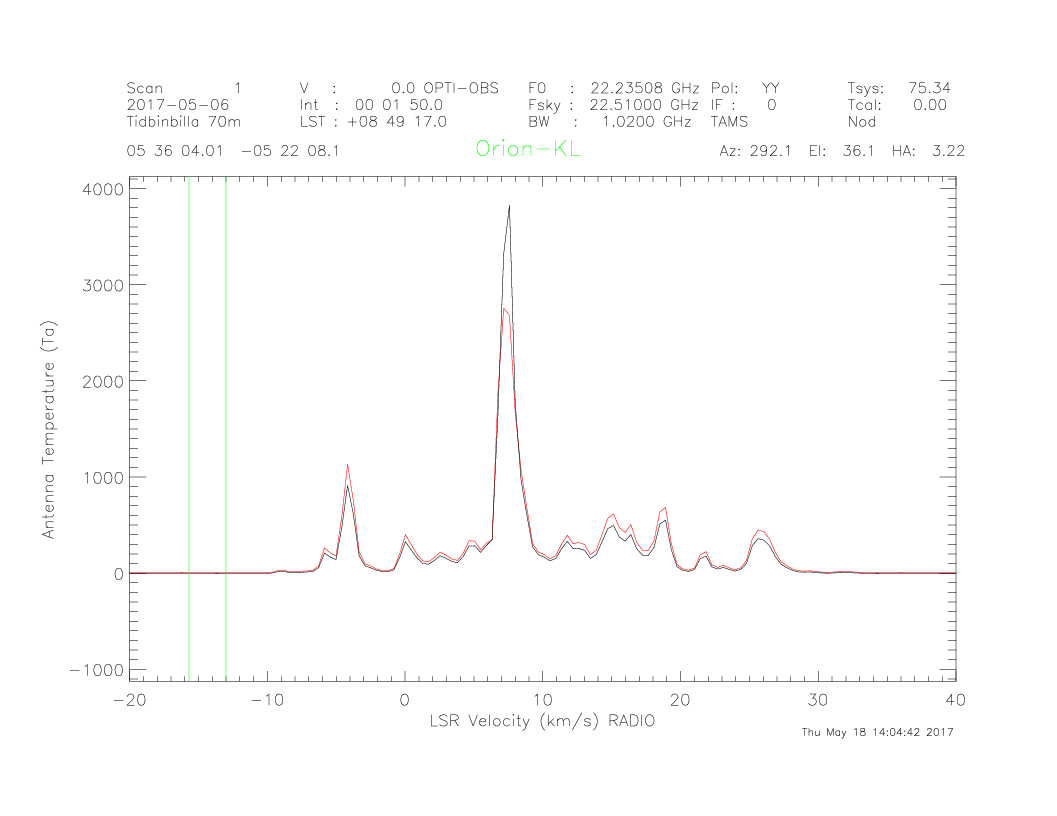
\includegraphics{Ori-H2O-obsCtrl.png}

.

Things to note are that * the Orion KL ICRS J2000 coordinates given by
SIMBAD are 05h35m14.16 -05d22'21.5" and the Orion A coordinates are
05h35m00.0 -05d20'00``, * assuming most of the features are unpolarized,
the polarizations are unbalanced by about 10\%, * the peak antenna
temperature is 3800K for the stronger polarization and 2700K for the
weaker. Bearing in mind the imbalance these could be about 4200K or
2400K respectively, depending on which pol is correct.

\section{Reduction Verification}\label{reduction-verification}

\subsection{Define Data Sets}\label{define-data-sets}

We will now examine the original data and go through the reduction step
by step. After sshfs mounting of ra,

    % Make sure that atleast 4 lines are below the HR
    \needspace{4\baselineskip}

    
        \vspace{6pt}
        \makebox[0.1\linewidth]{\smaller\hfill\tt\color{nbframe-in-prompt}In\hspace{4pt}{[}3{]}:\hspace{4pt}}\\*
        \vspace{-2.65\baselineskip}
        \begin{ColorVerbatim}
            \vspace{-0.7\baselineskip}
            \begin{Verbatim}[commandchars=\\\{\}]
\PY{k+kn}{import} \PY{n+nn}{h5py}
\PY{k+kn}{from} \PY{n+nn}{os.path} \PY{k+kn}{import} \PY{n}{basename}
\PY{k+kn}{from} \PY{n+nn}{pylab} \PY{k+kn}{import} \PY{o}{*}

\PY{k+kn}{from} \PY{n+nn}{MonitorControl.BackEnds.ROACH1.SAOspec} \PY{k+kn}{import} \PY{n}{SAOhdf5}

\PY{n}{filename} \PY{o}{=} \PY{l+s}{\PYZdq{}}\PY{l+s}{/home/kuiper/mnt/ra/usr/local/RA\PYZus{}data/HDF5/dss43/2017/126/A2LiP1I1494057349.22.Orion\PYZhy{}KL.spec.h5}\PY{l+s}{\PYZdq{}}
\PY{n}{data} \PY{o}{=} \PY{n}{SAOhdf5}\PY{p}{(}\PY{n}{filename}\PY{p}{)}
\end{Verbatim}

            
                \vspace{-0.2\baselineskip}
            
        \end{ColorVerbatim}
    
Now we define the raw spectra.

    % Make sure that atleast 4 lines are below the HR
    \needspace{4\baselineskip}

    
        \vspace{6pt}
        \makebox[0.1\linewidth]{\smaller\hfill\tt\color{nbframe-in-prompt}In\hspace{4pt}{[}4{]}:\hspace{4pt}}\\*
        \vspace{-2.65\baselineskip}
        \begin{ColorVerbatim}
            \vspace{-0.7\baselineskip}
            \begin{Verbatim}[commandchars=\\\{\}]
\PY{c}{\PYZsh{} raw spectra source in beam 1}
\PY{n}{specA1P1sc1} \PY{o}{=} \PY{n}{data}\PY{o}{.}\PY{n}{data}\PY{p}{[}\PY{l+s}{\PYZsq{}}\PY{l+s}{spectraCh1}\PY{l+s}{\PYZsq{}}\PY{p}{]}\PY{p}{[}\PY{l+m+mi}{18}\PY{p}{,}\PY{p}{:}\PY{p}{]} \PY{c}{\PYZsh{} on}
\PY{n}{specA2P1sc1} \PY{o}{=} \PY{n}{data}\PY{o}{.}\PY{n}{data}\PY{p}{[}\PY{l+s}{\PYZsq{}}\PY{l+s}{spectraCh2}\PY{l+s}{\PYZsq{}}\PY{p}{]}\PY{p}{[}\PY{l+m+mi}{18}\PY{p}{,}\PY{p}{:}\PY{p}{]} \PY{c}{\PYZsh{} off}
\PY{n}{specA1P2sc1} \PY{o}{=} \PY{n}{data}\PY{o}{.}\PY{n}{data}\PY{p}{[}\PY{l+s}{\PYZsq{}}\PY{l+s}{spectraCh3}\PY{l+s}{\PYZsq{}}\PY{p}{]}\PY{p}{[}\PY{l+m+mi}{18}\PY{p}{,}\PY{p}{:}\PY{p}{]} \PY{c}{\PYZsh{} on}
\PY{n}{specA2P2sc1} \PY{o}{=} \PY{n}{data}\PY{o}{.}\PY{n}{data}\PY{p}{[}\PY{l+s}{\PYZsq{}}\PY{l+s}{spectraCh4}\PY{l+s}{\PYZsq{}}\PY{p}{]}\PY{p}{[}\PY{l+m+mi}{18}\PY{p}{,}\PY{p}{:}\PY{p}{]} \PY{c}{\PYZsh{} off}
\PY{c}{\PYZsh{} raw spectra source in beam 2}
\PY{n}{specA1P1sc2} \PY{o}{=} \PY{n}{data}\PY{o}{.}\PY{n}{data}\PY{p}{[}\PY{l+s}{\PYZsq{}}\PY{l+s}{spectraCh1}\PY{l+s}{\PYZsq{}}\PY{p}{]}\PY{p}{[}\PY{l+m+mi}{44}\PY{p}{,}\PY{p}{:}\PY{p}{]} \PY{c}{\PYZsh{} off}
\PY{n}{specA2P1sc2} \PY{o}{=} \PY{n}{data}\PY{o}{.}\PY{n}{data}\PY{p}{[}\PY{l+s}{\PYZsq{}}\PY{l+s}{spectraCh2}\PY{l+s}{\PYZsq{}}\PY{p}{]}\PY{p}{[}\PY{l+m+mi}{44}\PY{p}{,}\PY{p}{:}\PY{p}{]} \PY{c}{\PYZsh{} on}
\PY{n}{specA1P2sc2} \PY{o}{=} \PY{n}{data}\PY{o}{.}\PY{n}{data}\PY{p}{[}\PY{l+s}{\PYZsq{}}\PY{l+s}{spectraCh3}\PY{l+s}{\PYZsq{}}\PY{p}{]}\PY{p}{[}\PY{l+m+mi}{44}\PY{p}{,}\PY{p}{:}\PY{p}{]} \PY{c}{\PYZsh{} off}
\PY{n}{specA2P2sc2} \PY{o}{=} \PY{n}{data}\PY{o}{.}\PY{n}{data}\PY{p}{[}\PY{l+s}{\PYZsq{}}\PY{l+s}{spectraCh4}\PY{l+s}{\PYZsq{}}\PY{p}{]}\PY{p}{[}\PY{l+m+mi}{44}\PY{p}{,}\PY{p}{:}\PY{p}{]} \PY{c}{\PYZsh{} on}
\end{Verbatim}

            
                \vspace{-0.2\baselineskip}
            
        \end{ColorVerbatim}
    
\subsection{Inspection of Data}\label{inspection-of-data}

First of all, let's examine the individual raw spectra.

    % Make sure that atleast 4 lines are below the HR
    \needspace{4\baselineskip}

    
        \vspace{6pt}
        \makebox[0.1\linewidth]{\smaller\hfill\tt\color{nbframe-in-prompt}In\hspace{4pt}{[}5{]}:\hspace{4pt}}\\*
        \vspace{-2.65\baselineskip}
        \begin{ColorVerbatim}
            \vspace{-0.7\baselineskip}
            \begin{Verbatim}[commandchars=\\\{\}]
\PY{n}{fig}\PY{p}{,} \PY{n}{ax} \PY{o}{=} \PY{n}{subplots}\PY{p}{(}\PY{n}{nrows}\PY{o}{=}\PY{l+m+mi}{1}\PY{p}{,}\PY{n}{ncols}\PY{o}{=}\PY{l+m+mi}{2}\PY{p}{,}\PY{n}{figsize}\PY{o}{=}\PY{p}{(}\PY{l+m+mi}{16}\PY{p}{,}\PY{l+m+mi}{6}\PY{p}{)}\PY{p}{)}
\PY{n}{ax}\PY{p}{[}\PY{l+m+mi}{0}\PY{p}{]}\PY{o}{.}\PY{n}{semilogy}\PY{p}{(}\PY{n}{specA1P1sc1}\PY{p}{,}\PY{n}{label}\PY{o}{=}\PY{l+s}{\PYZdq{}}\PY{l+s}{Ch1}\PY{l+s}{\PYZdq{}}\PY{p}{)} \PY{c}{\PYZsh{} A1P1}
\PY{n}{ax}\PY{p}{[}\PY{l+m+mi}{0}\PY{p}{]}\PY{o}{.}\PY{n}{semilogy}\PY{p}{(}\PY{n}{specA2P1sc1}\PY{p}{,}\PY{n}{label}\PY{o}{=}\PY{l+s}{\PYZdq{}}\PY{l+s}{Ch2}\PY{l+s}{\PYZdq{}}\PY{p}{)} \PY{c}{\PYZsh{} A2P1}
\PY{n}{ax}\PY{p}{[}\PY{l+m+mi}{0}\PY{p}{]}\PY{o}{.}\PY{n}{semilogy}\PY{p}{(}\PY{n}{specA1P2sc1}\PY{p}{,}\PY{n}{label}\PY{o}{=}\PY{l+s}{\PYZdq{}}\PY{l+s}{Ch3}\PY{l+s}{\PYZdq{}}\PY{p}{)} \PY{c}{\PYZsh{} A1P2}
\PY{n}{ax}\PY{p}{[}\PY{l+m+mi}{0}\PY{p}{]}\PY{o}{.}\PY{n}{semilogy}\PY{p}{(}\PY{n}{specA2P2sc1}\PY{p}{,}\PY{n}{label}\PY{o}{=}\PY{l+s}{\PYZdq{}}\PY{l+s}{Ch4}\PY{l+s}{\PYZdq{}}\PY{p}{)} \PY{c}{\PYZsh{} A2P2}
\PY{n}{ax}\PY{p}{[}\PY{l+m+mi}{0}\PY{p}{]}\PY{o}{.}\PY{n}{set\PYZus{}xlim}\PY{p}{(}\PY{l+m+mi}{7300}\PY{p}{,}\PY{l+m+mi}{7600}\PY{p}{)}
\PY{n}{ax}\PY{p}{[}\PY{l+m+mi}{0}\PY{p}{]}\PY{o}{.}\PY{n}{set\PYZus{}ylim}\PY{p}{(}\PY{l+m+mf}{1e6}\PY{p}{,}\PY{l+m+mf}{1e9}\PY{p}{)}
\PY{n}{ax}\PY{p}{[}\PY{l+m+mi}{0}\PY{p}{]}\PY{o}{.}\PY{n}{set\PYZus{}title}\PY{p}{(}\PY{l+s}{\PYZdq{}}\PY{l+s}{Raw spectra scan 1, record 18}\PY{l+s}{\PYZdq{}}\PY{p}{)}
\PY{n}{ax}\PY{p}{[}\PY{l+m+mi}{0}\PY{p}{]}\PY{o}{.}\PY{n}{grid}\PY{p}{(}\PY{n+nb+bp}{True}\PY{p}{)}
\PY{n}{ax}\PY{p}{[}\PY{l+m+mi}{0}\PY{p}{]}\PY{o}{.}\PY{n}{legend}\PY{p}{(}\PY{p}{)}
\PY{n}{ax}\PY{p}{[}\PY{l+m+mi}{0}\PY{p}{]}\PY{o}{.}\PY{n}{text}\PY{p}{(}\PY{l+m+mi}{7250}\PY{p}{,}\PY{l+m+mf}{3e8}\PY{p}{,}\PY{n}{data}\PY{o}{.}\PY{n}{data}\PY{p}{[}\PY{l+s}{\PYZsq{}}\PY{l+s}{mode}\PY{l+s}{\PYZsq{}}\PY{p}{]}\PY{p}{[}\PY{l+m+mi}{18}\PY{p}{]}\PY{p}{)}
\PY{n}{ax}\PY{p}{[}\PY{l+m+mi}{1}\PY{p}{]}\PY{o}{.}\PY{n}{semilogy}\PY{p}{(}\PY{n}{specA1P1sc2}\PY{p}{,}\PY{n}{label}\PY{o}{=}\PY{l+s}{\PYZdq{}}\PY{l+s}{Ch1}\PY{l+s}{\PYZdq{}}\PY{p}{)}
\PY{n}{ax}\PY{p}{[}\PY{l+m+mi}{1}\PY{p}{]}\PY{o}{.}\PY{n}{semilogy}\PY{p}{(}\PY{n}{specA2P1sc2}\PY{p}{,}\PY{n}{label}\PY{o}{=}\PY{l+s}{\PYZdq{}}\PY{l+s}{Ch2}\PY{l+s}{\PYZdq{}}\PY{p}{)}
\PY{n}{ax}\PY{p}{[}\PY{l+m+mi}{1}\PY{p}{]}\PY{o}{.}\PY{n}{semilogy}\PY{p}{(}\PY{n}{specA1P2sc2}\PY{p}{,}\PY{n}{label}\PY{o}{=}\PY{l+s}{\PYZdq{}}\PY{l+s}{Ch3}\PY{l+s}{\PYZdq{}}\PY{p}{)}
\PY{n}{ax}\PY{p}{[}\PY{l+m+mi}{1}\PY{p}{]}\PY{o}{.}\PY{n}{semilogy}\PY{p}{(}\PY{n}{specA2P2sc2}\PY{p}{,}\PY{n}{label}\PY{o}{=}\PY{l+s}{\PYZdq{}}\PY{l+s}{Ch4}\PY{l+s}{\PYZdq{}}\PY{p}{)}
\PY{n}{ax}\PY{p}{[}\PY{l+m+mi}{1}\PY{p}{]}\PY{o}{.}\PY{n}{set\PYZus{}xlim}\PY{p}{(}\PY{l+m+mi}{7300}\PY{p}{,}\PY{l+m+mi}{7600}\PY{p}{)}
\PY{n}{ax}\PY{p}{[}\PY{l+m+mi}{1}\PY{p}{]}\PY{o}{.}\PY{n}{set\PYZus{}ylim}\PY{p}{(}\PY{l+m+mf}{1e6}\PY{p}{,}\PY{l+m+mf}{1e9}\PY{p}{)}
\PY{n}{ax}\PY{p}{[}\PY{l+m+mi}{1}\PY{p}{]}\PY{o}{.}\PY{n}{set\PYZus{}title}\PY{p}{(}\PY{l+s}{\PYZdq{}}\PY{l+s}{Raw spectra scan 2, record 44}\PY{l+s}{\PYZdq{}}\PY{p}{)}
\PY{n}{ax}\PY{p}{[}\PY{l+m+mi}{1}\PY{p}{]}\PY{o}{.}\PY{n}{grid}\PY{p}{(}\PY{n+nb+bp}{True}\PY{p}{)}
\PY{n}{ax}\PY{p}{[}\PY{l+m+mi}{1}\PY{p}{]}\PY{o}{.}\PY{n}{legend}\PY{p}{(}\PY{p}{)}
\PY{n}{ax}\PY{p}{[}\PY{l+m+mi}{1}\PY{p}{]}\PY{o}{.}\PY{n}{text}\PY{p}{(}\PY{l+m+mi}{7250}\PY{p}{,}\PY{l+m+mf}{3e8}\PY{p}{,}\PY{n}{data}\PY{o}{.}\PY{n}{data}\PY{p}{[}\PY{l+s}{\PYZsq{}}\PY{l+s}{mode}\PY{l+s}{\PYZsq{}}\PY{p}{]}\PY{p}{[}\PY{l+m+mi}{44}\PY{p}{]}\PY{p}{)}
\PY{n}{fig}\PY{o}{.}\PY{n}{suptitle}\PY{p}{(}\PY{n}{basename}\PY{p}{(}\PY{n}{filename}\PY{p}{)}\PY{p}{)}
\PY{n}{show}\PY{p}{(}\PY{p}{)}
\end{Verbatim}

            
                \vspace{-0.2\baselineskip}
            
        \end{ColorVerbatim}
    

    

        % If the first block is an image, minipage the image.  Else
        % request a certain amount of space for the input text.
        \needspace{4\baselineskip}
        
        

            % Add document contents.
            
                \begin{InvisibleVerbatim}
                \vspace{-0.5\baselineskip}
    \begin{center}
    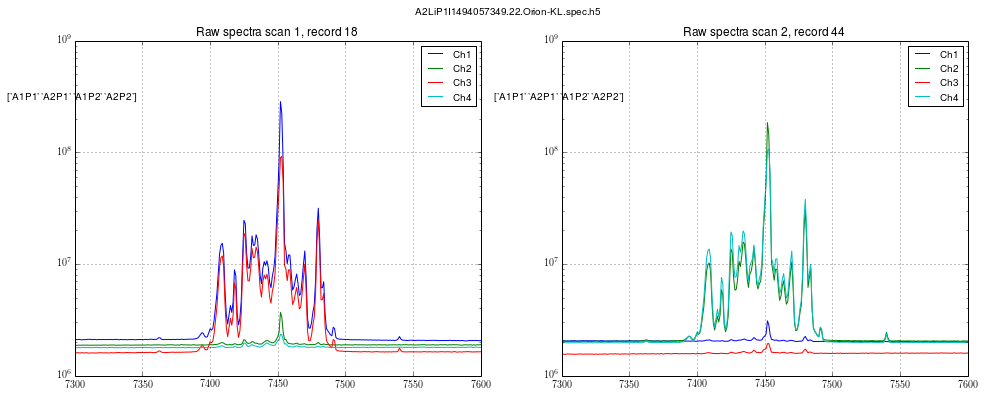
\includegraphics[max size={\textwidth}{\textheight}]{K-Band Calibration and Reduction_files/K-Band Calibration and Reduction_7_0.png}
    \par
    \end{center}
    
            \end{InvisibleVerbatim}
            
        
    
From this we can conclude that * Ch.1 and Ch.3 are from beam 1 (A1) and
Ch.2 and Ch.4 are from beam 2 (A2), * Ch.1 and Ch.3 are pretty well
balanced, assuming most of the features are unpolarized and noting the
baseline offset, * Ch.2 seems to be about 10\% weaker than Ch.4, and *
there is 1 or 2\% cross-polarization.

\subsection{Polarization Conversion}\label{polarization-conversion}

We can take ratios to see how well the polarization converting hybrids
are doing.

    % Make sure that atleast 4 lines are below the HR
    \needspace{4\baselineskip}

    
        \vspace{6pt}
        \makebox[0.1\linewidth]{\smaller\hfill\tt\color{nbframe-in-prompt}In\hspace{4pt}{[}6{]}:\hspace{4pt}}\\*
        \vspace{-2.65\baselineskip}
        \begin{ColorVerbatim}
            \vspace{-0.7\baselineskip}
            \begin{Verbatim}[commandchars=\\\{\}]
\PY{c}{\PYZsh{} ratios to compare polarizations}
\PY{n}{figure}\PY{p}{(}\PY{p}{)}
\PY{c}{\PYZsh{} A1P1/A1P2 scan 1}
\PY{n}{plot}\PY{p}{(}\PY{n}{specA1P1sc1}\PY{o}{/}\PY{n}{specA1P2sc1}\PY{p}{,} \PY{n}{label}\PY{o}{=}\PY{l+s}{\PYZdq{}}\PY{l+s}{Ch1/Ch3 A1}\PY{l+s}{\PYZdq{}}\PY{p}{)}
\PY{c}{\PYZsh{} A2P1/A2P2}
\PY{n}{plot}\PY{p}{(}\PY{n}{specA2P1sc2}\PY{o}{/}\PY{n}{specA2P2sc2}\PY{p}{,} \PY{n}{label}\PY{o}{=}\PY{l+s}{\PYZdq{}}\PY{l+s}{Ch2/Ch4 A2}\PY{l+s}{\PYZdq{}}\PY{p}{)}
\PY{n}{xlim}\PY{p}{(}\PY{l+m+mi}{7300}\PY{p}{,}\PY{l+m+mi}{7600}\PY{p}{)}
\PY{n}{ylim}\PY{p}{(}\PY{l+m+mi}{0}\PY{p}{,}\PY{l+m+mi}{4}\PY{p}{)}
\PY{n}{legend}\PY{p}{(}\PY{p}{)}
\PY{n}{grid}\PY{p}{(}\PY{p}{)}
\PY{n}{title}\PY{p}{(}\PY{l+s}{\PYZdq{}}\PY{l+s}{P1/P2 for same beam}\PY{l+s}{\PYZdq{}}\PY{p}{)}
\end{Verbatim}

            
                \vspace{-0.2\baselineskip}
            
        \end{ColorVerbatim}
    

    

        % If the first block is an image, minipage the image.  Else
        % request a certain amount of space for the input text.
        \needspace{4\baselineskip}
        
        

            % Add document contents.
            
                \begin{InvisibleVerbatim}
                \vspace{-0.5\baselineskip}
\begin{alltt}-c:4: RuntimeWarning: divide by zero encountered in divide
-c:4: RuntimeWarning: invalid value encountered in divide
\end{alltt}

            \end{InvisibleVerbatim}
            
                \makebox[0.1\linewidth]{\smaller\hfill\tt\color{nbframe-out-prompt}Out\hspace{4pt}{[}6{]}:\hspace{4pt}}\\*
                \vspace{-2.55\baselineskip}\begin{InvisibleVerbatim}
                \vspace{-0.5\baselineskip}
\begin{alltt}<matplotlib.text.Text at 0x7fdbadcfb250>\end{alltt}

            \end{InvisibleVerbatim}
            
                \begin{InvisibleVerbatim}
                \vspace{-0.5\baselineskip}
    \begin{center}
    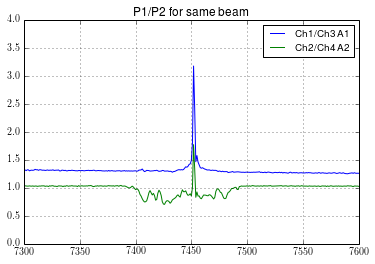
\includegraphics[max size={\textwidth}{\textheight}]{K-Band Calibration and Reduction_files/K-Band Calibration and Reduction_9_2.png}
    \par
    \end{center}
    
            \end{InvisibleVerbatim}
            
        
    
Assuming that most of the polarization is unpolarized, it would seem
that Ch.4 (A2P2) is too strong compared to Ch.2 (A2P1) or vice versa.

\subsection{Position Switched
Reduction}\label{position-switched-reduction}

Let's do the simplest form of data reduction first, which is position
switching. The source is in A1 during scan 1.

    % Make sure that atleast 4 lines are below the HR
    \needspace{4\baselineskip}

    
        \vspace{6pt}
        \makebox[0.1\linewidth]{\smaller\hfill\tt\color{nbframe-in-prompt}In\hspace{4pt}{[}7{]}:\hspace{4pt}}\\*
        \vspace{-2.65\baselineskip}
        \begin{ColorVerbatim}
            \vspace{-0.7\baselineskip}
            \begin{Verbatim}[commandchars=\\\{\}]
\PY{c}{\PYZsh{} position switching only}
\PY{n}{figure}\PY{p}{(}\PY{p}{)}
\PY{c}{\PYZsh{} pos 1 on}
\PY{n}{TsysP1sc1} \PY{o}{=} \PY{n}{data}\PY{o}{.}\PY{n}{data}\PY{p}{[}\PY{l+s}{\PYZsq{}}\PY{l+s}{Tsys}\PY{l+s}{\PYZsq{}}\PY{p}{]}\PY{p}{[}\PY{l+m+mi}{18}\PY{p}{]}\PY{p}{[}\PY{l+m+mi}{0}\PY{p}{]} \PY{c}{\PYZsh{} pol 1}
\PY{n}{TsysP2sc1} \PY{o}{=} \PY{n}{data}\PY{o}{.}\PY{n}{data}\PY{p}{[}\PY{l+s}{\PYZsq{}}\PY{l+s}{Tsys}\PY{l+s}{\PYZsq{}}\PY{p}{]}\PY{p}{[}\PY{l+m+mi}{18}\PY{p}{]}\PY{p}{[}\PY{l+m+mi}{2}\PY{p}{]} \PY{c}{\PYZsh{} pol 2}
\PY{c}{\PYZsh{} pos 2 off}
\PY{n}{TsysP1sc2} \PY{o}{=} \PY{n}{data}\PY{o}{.}\PY{n}{data}\PY{p}{[}\PY{l+s}{\PYZsq{}}\PY{l+s}{Tsys}\PY{l+s}{\PYZsq{}}\PY{p}{]}\PY{p}{[}\PY{l+m+mi}{44}\PY{p}{]}\PY{p}{[}\PY{l+m+mi}{0}\PY{p}{]}
\PY{n}{TsysP2sc2} \PY{o}{=} \PY{n}{data}\PY{o}{.}\PY{n}{data}\PY{p}{[}\PY{l+s}{\PYZsq{}}\PY{l+s}{Tsys}\PY{l+s}{\PYZsq{}}\PY{p}{]}\PY{p}{[}\PY{l+m+mi}{44}\PY{p}{]}\PY{p}{[}\PY{l+m+mi}{2}\PY{p}{]}
\PY{n}{ratioP1} \PY{o}{=} \PY{n}{specA1P1sc1}\PY{o}{/}\PY{n}{specA1P1sc2}
\PY{n}{ratioP2} \PY{o}{=} \PY{n}{specA1P2sc1}\PY{o}{/}\PY{n}{specA1P2sc2}
\PY{n}{plot}\PY{p}{(}\PY{n}{TsysP1sc2}\PY{o}{*}\PY{p}{(}\PY{n}{ratioP1} \PY{o}{\PYZhy{}} \PY{l+m+mi}{1}\PY{p}{)}\PY{p}{,} \PY{n}{label}\PY{o}{=}\PY{l+s}{\PYZdq{}}\PY{l+s}{pol 1}\PY{l+s}{\PYZdq{}}\PY{p}{)}
\PY{n}{plot}\PY{p}{(}\PY{n}{TsysP2sc2}\PY{o}{*}\PY{p}{(}\PY{n}{ratioP2} \PY{o}{\PYZhy{}} \PY{l+m+mi}{1}\PY{p}{)}\PY{p}{,} \PY{n}{label}\PY{o}{=}\PY{l+s}{\PYZdq{}}\PY{l+s}{pol 2}\PY{l+s}{\PYZdq{}}\PY{p}{)}
\PY{n}{legend}\PY{p}{(}\PY{p}{)}
\PY{n}{ylabel}\PY{p}{(}\PY{l+s}{\PYZdq{}}\PY{l+s}{Antenna Temperature}\PY{l+s}{\PYZdq{}}\PY{p}{)}
\PY{n}{grid}\PY{p}{(}\PY{p}{)}
\PY{n}{xlim}\PY{p}{(}\PY{l+m+mi}{7300}\PY{p}{,}\PY{l+m+mi}{7600}\PY{p}{)}
\PY{n}{ylim}\PY{p}{(}\PY{l+m+mi}{0}\PY{p}{,}\PY{l+m+mi}{6000}\PY{p}{)}
\PY{n}{title}\PY{p}{(}\PY{l+s}{\PYZdq{}}\PY{l+s}{Position switching only}\PY{l+s}{\PYZdq{}}\PY{p}{)}
\end{Verbatim}

            
                \vspace{-0.2\baselineskip}
            
        \end{ColorVerbatim}
    

    

        % If the first block is an image, minipage the image.  Else
        % request a certain amount of space for the input text.
        \needspace{4\baselineskip}
        
        

            % Add document contents.
            
                \begin{InvisibleVerbatim}
                \vspace{-0.5\baselineskip}
\begin{alltt}-c:9: RuntimeWarning: divide by zero encountered in divide
-c:10: RuntimeWarning: divide by zero encountered in divide
-c:10: RuntimeWarning: invalid value encountered in divide
\end{alltt}

            \end{InvisibleVerbatim}
            
                \makebox[0.1\linewidth]{\smaller\hfill\tt\color{nbframe-out-prompt}Out\hspace{4pt}{[}7{]}:\hspace{4pt}}\\*
                \vspace{-2.55\baselineskip}\begin{InvisibleVerbatim}
                \vspace{-0.5\baselineskip}
\begin{alltt}<matplotlib.text.Text at 0x7fdbac3c4850>\end{alltt}

            \end{InvisibleVerbatim}
            
                \begin{InvisibleVerbatim}
                \vspace{-0.5\baselineskip}
    \begin{center}
    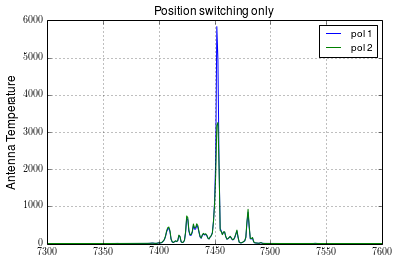
\includegraphics[max size={\textwidth}{\textheight}]{K-Band Calibration and Reduction_files/K-Band Calibration and Reduction_11_2.png}
    \par
    \end{center}
    
            \end{InvisibleVerbatim}
            
        
    
We have a result which is well-balanced for most of the features. The
main components shows strong polarization. Comparing this to Shinji's
spectrum bear in mind that his is plotted as a function of radial
velocity while the above is in channel number. We note that * the
antenna temperatures of the second strongest feature is the same here
are for P1 in Shinji's spectrum, about 900K, * the antenna temperatures
of the main feature are stronger, 5900 vs 3800 for P1 and 3200 vs 2800
for P2. We need to bear in mind that our result uses only one ON record
and one OFF record but still, one would not expect the average to be
very different unless the pointing was poor.

We can check on this by selecting a record near the end of each scan.

    % Make sure that atleast 4 lines are below the HR
    \needspace{4\baselineskip}

    
        \vspace{6pt}
        \makebox[0.1\linewidth]{\smaller\hfill\tt\color{nbframe-in-prompt}In\hspace{4pt}{[}8{]}:\hspace{4pt}}\\*
        \vspace{-2.65\baselineskip}
        \begin{ColorVerbatim}
            \vspace{-0.7\baselineskip}
            \begin{Verbatim}[commandchars=\\\{\}]
\PY{k}{print} \PY{l+s}{\PYZdq{}}\PY{l+s}{ 0 \PYZhy{} 10}\PY{l+s+se}{\PYZbs{}n}\PY{l+s}{\PYZdq{}}\PY{p}{,}\PY{n}{data}\PY{o}{.}\PY{n}{data}\PY{p}{[}\PY{l+s}{\PYZsq{}}\PY{l+s}{scan\PYZus{}number}\PY{l+s}{\PYZsq{}}\PY{p}{]}\PY{p}{[}\PY{l+m+mi}{0}\PY{p}{:}\PY{l+m+mi}{10}\PY{p}{]}
\PY{k}{print} \PY{l+s}{\PYZdq{}}\PY{l+s}{10 \PYZhy{} 20}\PY{l+s+se}{\PYZbs{}n}\PY{l+s}{\PYZdq{}}\PY{p}{,}\PY{n}{data}\PY{o}{.}\PY{n}{data}\PY{p}{[}\PY{l+s}{\PYZsq{}}\PY{l+s}{scan\PYZus{}number}\PY{l+s}{\PYZsq{}}\PY{p}{]}\PY{p}{[}\PY{l+m+mi}{10}\PY{p}{:}\PY{l+m+mi}{20}\PY{p}{]}
\PY{k}{print} \PY{l+s}{\PYZdq{}}\PY{l+s}{20 \PYZhy{} 30}\PY{l+s+se}{\PYZbs{}n}\PY{l+s}{\PYZdq{}}\PY{p}{,}\PY{n}{data}\PY{o}{.}\PY{n}{data}\PY{p}{[}\PY{l+s}{\PYZsq{}}\PY{l+s}{scan\PYZus{}number}\PY{l+s}{\PYZsq{}}\PY{p}{]}\PY{p}{[}\PY{l+m+mi}{20}\PY{p}{:}\PY{l+m+mi}{30}\PY{p}{]}
\PY{k}{print} \PY{l+s}{\PYZdq{}}\PY{l+s}{30 \PYZhy{} 40}\PY{l+s+se}{\PYZbs{}n}\PY{l+s}{\PYZdq{}}\PY{p}{,}\PY{n}{data}\PY{o}{.}\PY{n}{data}\PY{p}{[}\PY{l+s}{\PYZsq{}}\PY{l+s}{scan\PYZus{}number}\PY{l+s}{\PYZsq{}}\PY{p}{]}\PY{p}{[}\PY{l+m+mi}{30}\PY{p}{:}\PY{l+m+mi}{40}\PY{p}{]}
\PY{k}{print} \PY{l+s}{\PYZdq{}}\PY{l+s}{40 \PYZhy{} 50}\PY{l+s+se}{\PYZbs{}n}\PY{l+s}{\PYZdq{}}\PY{p}{,}\PY{n}{data}\PY{o}{.}\PY{n}{data}\PY{p}{[}\PY{l+s}{\PYZsq{}}\PY{l+s}{scan\PYZus{}number}\PY{l+s}{\PYZsq{}}\PY{p}{]}\PY{p}{[}\PY{l+m+mi}{40}\PY{p}{:}\PY{l+m+mi}{50}\PY{p}{]}
\PY{k}{print} \PY{l+s}{\PYZdq{}}\PY{l+s}{50 \PYZhy{} 60}\PY{l+s+se}{\PYZbs{}n}\PY{l+s}{\PYZdq{}}\PY{p}{,}\PY{n}{data}\PY{o}{.}\PY{n}{data}\PY{p}{[}\PY{l+s}{\PYZsq{}}\PY{l+s}{scan\PYZus{}number}\PY{l+s}{\PYZsq{}}\PY{p}{]}\PY{p}{[}\PY{l+m+mi}{50}\PY{p}{:}\PY{l+m+mi}{60}\PY{p}{]}
\PY{k}{print} \PY{l+s}{\PYZdq{}}\PY{l+s}{60 \PYZhy{} 70}\PY{l+s+se}{\PYZbs{}n}\PY{l+s}{\PYZdq{}}\PY{p}{,}\PY{n}{data}\PY{o}{.}\PY{n}{data}\PY{p}{[}\PY{l+s}{\PYZsq{}}\PY{l+s}{scan\PYZus{}number}\PY{l+s}{\PYZsq{}}\PY{p}{]}\PY{p}{[}\PY{l+m+mi}{60}\PY{p}{:}\PY{l+m+mi}{70}\PY{p}{]}
\end{Verbatim}

            
                \vspace{-0.2\baselineskip}
            
        \end{ColorVerbatim}
    

    

        % If the first block is an image, minipage the image.  Else
        % request a certain amount of space for the input text.
        \needspace{4\baselineskip}
        
        

            % Add document contents.
            
                \begin{InvisibleVerbatim}
                \vspace{-0.5\baselineskip}
\begin{alltt} 0 - 10
[[-1.]
 [-1.]
 ...
 [-1.]
 [-1.]]
10 - 20
[[-1.]
 ...
 [-1.]
 [-1.]
 [ 1.]
 [ 1.]
 [ 1.]]
20 - 30
[[ 1.]
 [ 1.]
 ...
 [ 1.]
 [ 1.]]
30 - 40
[[ 1.]
 [ 1.]
 ...
 [ 1.]
 [ 1.]]
40 - 50
[[ 1.]
 [-1.]
 [-1.]
 [ 2.]
 [ 2.]
 ...
 [ 2.]
 [ 2.]]
50 - 60
[[ 2.]
 [ 2.]
 [ 2.]
 [ 2.]
 [ 2.]
 [ 2.]
 [ 2.]
 [ 2.]
 [ 2.]
 [ 2.]]
60 - 70
[[ 2.]
 [ 2.]
 ...
 [ 2.]
 [ 2.]
 [-1.]
 [ 0.]]
\end{alltt}

            \end{InvisibleVerbatim}
            
        
    
So instead of 18 and 44 let's take 39 and 65.

    % Make sure that atleast 4 lines are below the HR
    \needspace{4\baselineskip}

    
        \vspace{6pt}
        \makebox[0.1\linewidth]{\smaller\hfill\tt\color{nbframe-in-prompt}In\hspace{4pt}{[}9{]}:\hspace{4pt}}\\*
        \vspace{-2.65\baselineskip}
        \begin{ColorVerbatim}
            \vspace{-0.7\baselineskip}
            \begin{Verbatim}[commandchars=\\\{\}]
\PY{c}{\PYZsh{} position switching only}
\PY{n}{specA1P1sc1a} \PY{o}{=} \PY{n}{data}\PY{o}{.}\PY{n}{data}\PY{p}{[}\PY{l+s}{\PYZsq{}}\PY{l+s}{spectraCh1}\PY{l+s}{\PYZsq{}}\PY{p}{]}\PY{p}{[}\PY{l+m+mi}{39}\PY{p}{,}\PY{p}{:}\PY{p}{]}
\PY{n}{specA1P1sc2a} \PY{o}{=} \PY{n}{data}\PY{o}{.}\PY{n}{data}\PY{p}{[}\PY{l+s}{\PYZsq{}}\PY{l+s}{spectraCh1}\PY{l+s}{\PYZsq{}}\PY{p}{]}\PY{p}{[}\PY{l+m+mi}{65}\PY{p}{,}\PY{p}{:}\PY{p}{]}
\PY{n}{specA1P2sc1a} \PY{o}{=} \PY{n}{data}\PY{o}{.}\PY{n}{data}\PY{p}{[}\PY{l+s}{\PYZsq{}}\PY{l+s}{spectraCh3}\PY{l+s}{\PYZsq{}}\PY{p}{]}\PY{p}{[}\PY{l+m+mi}{39}\PY{p}{,}\PY{p}{:}\PY{p}{]}
\PY{n}{specA1P2sc2a} \PY{o}{=} \PY{n}{data}\PY{o}{.}\PY{n}{data}\PY{p}{[}\PY{l+s}{\PYZsq{}}\PY{l+s}{spectraCh3}\PY{l+s}{\PYZsq{}}\PY{p}{]}\PY{p}{[}\PY{l+m+mi}{65}\PY{p}{,}\PY{p}{:}\PY{p}{]}

\PY{n}{figure}\PY{p}{(}\PY{p}{)}
\PY{c}{\PYZsh{} pos 1 on}
\PY{n}{TsysP1sc1a} \PY{o}{=} \PY{n}{data}\PY{o}{.}\PY{n}{data}\PY{p}{[}\PY{l+s}{\PYZsq{}}\PY{l+s}{Tsys}\PY{l+s}{\PYZsq{}}\PY{p}{]}\PY{p}{[}\PY{l+m+mi}{39}\PY{p}{]}\PY{p}{[}\PY{l+m+mi}{0}\PY{p}{]} \PY{c}{\PYZsh{} pol 1}
\PY{n}{TsysP2sc1a} \PY{o}{=} \PY{n}{data}\PY{o}{.}\PY{n}{data}\PY{p}{[}\PY{l+s}{\PYZsq{}}\PY{l+s}{Tsys}\PY{l+s}{\PYZsq{}}\PY{p}{]}\PY{p}{[}\PY{l+m+mi}{39}\PY{p}{]}\PY{p}{[}\PY{l+m+mi}{2}\PY{p}{]} \PY{c}{\PYZsh{} pol 2}
\PY{c}{\PYZsh{} pos 2 off}
\PY{n}{TsysP1sc2a} \PY{o}{=} \PY{n}{data}\PY{o}{.}\PY{n}{data}\PY{p}{[}\PY{l+s}{\PYZsq{}}\PY{l+s}{Tsys}\PY{l+s}{\PYZsq{}}\PY{p}{]}\PY{p}{[}\PY{l+m+mi}{65}\PY{p}{]}\PY{p}{[}\PY{l+m+mi}{0}\PY{p}{]}
\PY{n}{TsysP2sc2a} \PY{o}{=} \PY{n}{data}\PY{o}{.}\PY{n}{data}\PY{p}{[}\PY{l+s}{\PYZsq{}}\PY{l+s}{Tsys}\PY{l+s}{\PYZsq{}}\PY{p}{]}\PY{p}{[}\PY{l+m+mi}{65}\PY{p}{]}\PY{p}{[}\PY{l+m+mi}{2}\PY{p}{]}

\PY{n}{ratioP1a} \PY{o}{=} \PY{n}{specA1P1sc1a}\PY{o}{/}\PY{n}{specA1P1sc2a}
\PY{n}{ratioP2a} \PY{o}{=} \PY{n}{specA1P2sc1a}\PY{o}{/}\PY{n}{specA1P2sc2a}
\PY{n}{plot}\PY{p}{(}\PY{n}{TsysP1sc2a}\PY{o}{*}\PY{p}{(}\PY{n}{ratioP1a} \PY{o}{\PYZhy{}} \PY{l+m+mi}{1}\PY{p}{)}\PY{p}{,} \PY{n}{label}\PY{o}{=}\PY{l+s}{\PYZdq{}}\PY{l+s}{pol 1}\PY{l+s}{\PYZdq{}}\PY{p}{)}
\PY{n}{plot}\PY{p}{(}\PY{n}{TsysP2sc2a}\PY{o}{*}\PY{p}{(}\PY{n}{ratioP2a} \PY{o}{\PYZhy{}} \PY{l+m+mi}{1}\PY{p}{)}\PY{p}{,} \PY{n}{label}\PY{o}{=}\PY{l+s}{\PYZdq{}}\PY{l+s}{pol 2}\PY{l+s}{\PYZdq{}}\PY{p}{)}
\PY{n}{legend}\PY{p}{(}\PY{p}{)}
\PY{n}{ylabel}\PY{p}{(}\PY{l+s}{\PYZdq{}}\PY{l+s}{Antenna Temperature}\PY{l+s}{\PYZdq{}}\PY{p}{)}
\PY{n}{grid}\PY{p}{(}\PY{p}{)}
\PY{n}{xlim}\PY{p}{(}\PY{l+m+mi}{7300}\PY{p}{,}\PY{l+m+mi}{7600}\PY{p}{)}
\PY{n}{ylim}\PY{p}{(}\PY{l+m+mi}{0}\PY{p}{,}\PY{l+m+mi}{6000}\PY{p}{)}
\PY{n}{title}\PY{p}{(}\PY{l+s}{\PYZdq{}}\PY{l+s}{Position switching only}\PY{l+s}{\PYZdq{}}\PY{p}{)}
\end{Verbatim}

            
                \vspace{-0.2\baselineskip}
            
        \end{ColorVerbatim}
    

    

        % If the first block is an image, minipage the image.  Else
        % request a certain amount of space for the input text.
        \needspace{4\baselineskip}
        
        

            % Add document contents.
            
                \begin{InvisibleVerbatim}
                \vspace{-0.5\baselineskip}
\begin{alltt}-c:15: RuntimeWarning: divide by zero encountered in divide
-c:16: RuntimeWarning: divide by zero encountered in divide
-c:16: RuntimeWarning: invalid value encountered in divide
\end{alltt}

            \end{InvisibleVerbatim}
            
                \makebox[0.1\linewidth]{\smaller\hfill\tt\color{nbframe-out-prompt}Out\hspace{4pt}{[}9{]}:\hspace{4pt}}\\*
                \vspace{-2.55\baselineskip}\begin{InvisibleVerbatim}
                \vspace{-0.5\baselineskip}
\begin{alltt}<matplotlib.text.Text at 0x7fdbac315a50>\end{alltt}

            \end{InvisibleVerbatim}
            
                \begin{InvisibleVerbatim}
                \vspace{-0.5\baselineskip}
    \begin{center}
    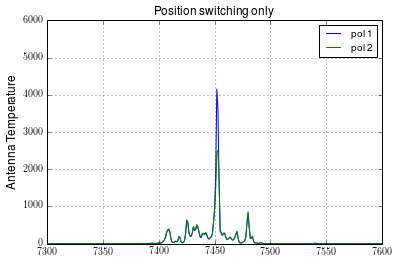
\includegraphics[max size={\textwidth}{\textheight}]{K-Band Calibration and Reduction_files/K-Band Calibration and Reduction_15_2.png}
    \par
    \end{center}
    
            \end{InvisibleVerbatim}
            
        
    
So that is quite a bit different and more like what Shinji has, 4100 vs
3800 and 2500 vs 2800. Might as well do one more from the middle of each
scan.

    % Make sure that atleast 4 lines are below the HR
    \needspace{4\baselineskip}

    
        \vspace{6pt}
        \makebox[0.1\linewidth]{\smaller\hfill\tt\color{nbframe-in-prompt}In\hspace{4pt}{[}10{]}:\hspace{4pt}}\\*
        \vspace{-2.65\baselineskip}
        \begin{ColorVerbatim}
            \vspace{-0.7\baselineskip}
            \begin{Verbatim}[commandchars=\\\{\}]
\PY{c}{\PYZsh{} position switching only}
\PY{n}{specA1P1sc1b} \PY{o}{=} \PY{n}{data}\PY{o}{.}\PY{n}{data}\PY{p}{[}\PY{l+s}{\PYZsq{}}\PY{l+s}{spectraCh1}\PY{l+s}{\PYZsq{}}\PY{p}{]}\PY{p}{[}\PY{l+m+mi}{28}\PY{p}{,}\PY{p}{:}\PY{p}{]}
\PY{n}{specA1P1sc2b} \PY{o}{=} \PY{n}{data}\PY{o}{.}\PY{n}{data}\PY{p}{[}\PY{l+s}{\PYZsq{}}\PY{l+s}{spectraCh1}\PY{l+s}{\PYZsq{}}\PY{p}{]}\PY{p}{[}\PY{l+m+mi}{54}\PY{p}{,}\PY{p}{:}\PY{p}{]}
\PY{n}{specA1P2sc1b} \PY{o}{=} \PY{n}{data}\PY{o}{.}\PY{n}{data}\PY{p}{[}\PY{l+s}{\PYZsq{}}\PY{l+s}{spectraCh3}\PY{l+s}{\PYZsq{}}\PY{p}{]}\PY{p}{[}\PY{l+m+mi}{28}\PY{p}{,}\PY{p}{:}\PY{p}{]}
\PY{n}{specA1P2sc2b} \PY{o}{=} \PY{n}{data}\PY{o}{.}\PY{n}{data}\PY{p}{[}\PY{l+s}{\PYZsq{}}\PY{l+s}{spectraCh3}\PY{l+s}{\PYZsq{}}\PY{p}{]}\PY{p}{[}\PY{l+m+mi}{54}\PY{p}{,}\PY{p}{:}\PY{p}{]}

\PY{n}{figure}\PY{p}{(}\PY{p}{)}
\PY{c}{\PYZsh{} pos 1 on}
\PY{n}{TsysP1sc1b} \PY{o}{=} \PY{n}{data}\PY{o}{.}\PY{n}{data}\PY{p}{[}\PY{l+s}{\PYZsq{}}\PY{l+s}{Tsys}\PY{l+s}{\PYZsq{}}\PY{p}{]}\PY{p}{[}\PY{l+m+mi}{28}\PY{p}{]}\PY{p}{[}\PY{l+m+mi}{0}\PY{p}{]} \PY{c}{\PYZsh{} pol 1}
\PY{n}{TsysP2sc1b} \PY{o}{=} \PY{n}{data}\PY{o}{.}\PY{n}{data}\PY{p}{[}\PY{l+s}{\PYZsq{}}\PY{l+s}{Tsys}\PY{l+s}{\PYZsq{}}\PY{p}{]}\PY{p}{[}\PY{l+m+mi}{54}\PY{p}{]}\PY{p}{[}\PY{l+m+mi}{2}\PY{p}{]} \PY{c}{\PYZsh{} pol 2}
\PY{c}{\PYZsh{} pos 2 off}
\PY{n}{TsysP1sc2b} \PY{o}{=} \PY{n}{data}\PY{o}{.}\PY{n}{data}\PY{p}{[}\PY{l+s}{\PYZsq{}}\PY{l+s}{Tsys}\PY{l+s}{\PYZsq{}}\PY{p}{]}\PY{p}{[}\PY{l+m+mi}{28}\PY{p}{]}\PY{p}{[}\PY{l+m+mi}{0}\PY{p}{]}
\PY{n}{TsysP2sc2b} \PY{o}{=} \PY{n}{data}\PY{o}{.}\PY{n}{data}\PY{p}{[}\PY{l+s}{\PYZsq{}}\PY{l+s}{Tsys}\PY{l+s}{\PYZsq{}}\PY{p}{]}\PY{p}{[}\PY{l+m+mi}{54}\PY{p}{]}\PY{p}{[}\PY{l+m+mi}{2}\PY{p}{]}

\PY{n}{ratioP1b} \PY{o}{=} \PY{n}{specA1P1sc1b}\PY{o}{/}\PY{n}{specA1P1sc2b}
\PY{n}{ratioP2b} \PY{o}{=} \PY{n}{specA1P2sc1b}\PY{o}{/}\PY{n}{specA1P2sc2b}
\PY{n}{plot}\PY{p}{(}\PY{n}{TsysP1sc2b}\PY{o}{*}\PY{p}{(}\PY{n}{ratioP1b} \PY{o}{\PYZhy{}} \PY{l+m+mi}{1}\PY{p}{)}\PY{p}{,} \PY{n}{label}\PY{o}{=}\PY{l+s}{\PYZdq{}}\PY{l+s}{pol 1}\PY{l+s}{\PYZdq{}}\PY{p}{)}
\PY{n}{plot}\PY{p}{(}\PY{n}{TsysP2sc2b}\PY{o}{*}\PY{p}{(}\PY{n}{ratioP2b} \PY{o}{\PYZhy{}} \PY{l+m+mi}{1}\PY{p}{)}\PY{p}{,} \PY{n}{label}\PY{o}{=}\PY{l+s}{\PYZdq{}}\PY{l+s}{pol 2}\PY{l+s}{\PYZdq{}}\PY{p}{)}
\PY{n}{legend}\PY{p}{(}\PY{p}{)}
\PY{n}{ylabel}\PY{p}{(}\PY{l+s}{\PYZdq{}}\PY{l+s}{Antenna Temperature}\PY{l+s}{\PYZdq{}}\PY{p}{)}
\PY{n}{grid}\PY{p}{(}\PY{p}{)}
\PY{n}{xlim}\PY{p}{(}\PY{l+m+mi}{7300}\PY{p}{,}\PY{l+m+mi}{7600}\PY{p}{)}
\PY{n}{ylim}\PY{p}{(}\PY{l+m+mi}{0}\PY{p}{,}\PY{l+m+mi}{6000}\PY{p}{)}
\PY{n}{title}\PY{p}{(}\PY{l+s}{\PYZdq{}}\PY{l+s}{Position switching only}\PY{l+s}{\PYZdq{}}\PY{p}{)}
\end{Verbatim}

            
                \vspace{-0.2\baselineskip}
            
        \end{ColorVerbatim}
    

    

        % If the first block is an image, minipage the image.  Else
        % request a certain amount of space for the input text.
        \needspace{4\baselineskip}
        
        

            % Add document contents.
            
                \makebox[0.1\linewidth]{\smaller\hfill\tt\color{nbframe-out-prompt}Out\hspace{4pt}{[}10{]}:\hspace{4pt}}\\*
                \vspace{-2.55\baselineskip}\begin{InvisibleVerbatim}
                \vspace{-0.5\baselineskip}
\begin{alltt}<matplotlib.text.Text at 0x7fdbac260d90>\end{alltt}

            \end{InvisibleVerbatim}
            
                \begin{InvisibleVerbatim}
                \vspace{-0.5\baselineskip}
    \begin{center}
    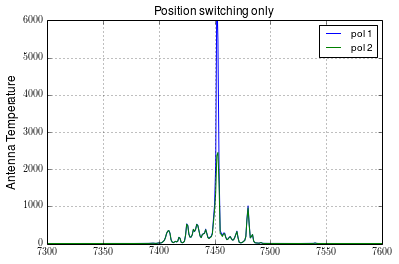
\includegraphics[max size={\textwidth}{\textheight}]{K-Band Calibration and Reduction_files/K-Band Calibration and Reduction_17_1.png}
    \par
    \end{center}
    
            \end{InvisibleVerbatim}
            
        
    
Clearly quite a lot of variation. Let's summarize in a table.

\begin{longtable}[c]{@{}ccccc@{}}
\hline %\toprule\addlinespace
Pol & Shinji & 18,44 & 29,54 & 39,65
\\%\addlinespace
\hline %%\midrule\endhead
1 & 3800 & 5900 & 6000 & 4100
\\%\addlinespace
2 & 2800 & 3200 & 2400 & 2500
\\%\addlinespace
ratio & 1.36 & 1.84 & 2.5 & 1.64
\\%\addlinespace
\hline%\bottomrule
\end{longtable}It's really hard to draw any conclusions from this, other than that the
pointing is probably quite poor.

\subsection{Beam and Position Switched
Reduction}\label{beam-and-position-switched-reduction}

\subsubsection{By Ratios}\label{by-ratios}

This method of reduction uses two beams, one on source and one off. The
on and off spectra are compared by taking a ratio. Then the other beam
is moved to the source and the process is repeated. The two ratios are
averaged and then scaled to system temperature.

    % Make sure that atleast 4 lines are below the HR
    \needspace{4\baselineskip}

    
        \vspace{6pt}
        \makebox[0.1\linewidth]{\smaller\hfill\tt\color{nbframe-in-prompt}In\hspace{4pt}{[}11{]}:\hspace{4pt}}\\*
        \vspace{-2.65\baselineskip}
        \begin{ColorVerbatim}
            \vspace{-0.7\baselineskip}
            \begin{Verbatim}[commandchars=\\\{\}]
\PY{c}{\PYZsh{} beam to beam ratio spectra, one for each pol}

\PY{c}{\PYZsh{} scan 1 on/off}
\PY{c}{\PYZsh{} pol 1}
\PY{n}{ratioP1sc1} \PY{o}{=} \PY{n}{specA1P1sc1}\PY{o}{/}\PY{n}{specA2P1sc1}
\PY{c}{\PYZsh{} pol 2}
\PY{n}{ratioP2sc1} \PY{o}{=} \PY{n}{specA1P2sc1}\PY{o}{/}\PY{n}{specA2P2sc1}

\PY{c}{\PYZsh{} scan 2 on/off}
\PY{c}{\PYZsh{} pol 1}
\PY{n}{ratioP1sc2} \PY{o}{=} \PY{n}{specA2P1sc2}\PY{o}{/}\PY{n}{specA1P1sc2}
\PY{c}{\PYZsh{} pol 2}
\PY{n}{ratioP2sc2} \PY{o}{=} \PY{n}{specA2P2sc2}\PY{o}{/}\PY{n}{specA1P2sc2}

\PY{n}{fig2}\PY{p}{,} \PY{n}{ax2} \PY{o}{=} \PY{n}{subplots}\PY{p}{(}\PY{n}{nrows}\PY{o}{=}\PY{l+m+mi}{1}\PY{p}{,}\PY{n}{ncols}\PY{o}{=}\PY{l+m+mi}{2}\PY{p}{,}\PY{n}{figsize}\PY{o}{=}\PY{p}{(}\PY{l+m+mi}{16}\PY{p}{,}\PY{l+m+mi}{6}\PY{p}{)}\PY{p}{)}
\PY{n}{ax2}\PY{p}{[}\PY{l+m+mi}{0}\PY{p}{]}\PY{o}{.}\PY{n}{plot}\PY{p}{(}\PY{n}{ratioP1sc1}\PY{p}{,} \PY{n}{label}\PY{o}{=}\PY{l+s}{\PYZdq{}}\PY{l+s}{Ch1/Ch2 P1}\PY{l+s}{\PYZdq{}}\PY{p}{)}
\PY{n}{ax2}\PY{p}{[}\PY{l+m+mi}{0}\PY{p}{]}\PY{o}{.}\PY{n}{plot}\PY{p}{(}\PY{n}{ratioP2sc1}\PY{p}{,} \PY{n}{label}\PY{o}{=}\PY{l+s}{\PYZdq{}}\PY{l+s}{Ch3/Ch4 P2}\PY{l+s}{\PYZdq{}}\PY{p}{)}
\PY{n}{ax2}\PY{p}{[}\PY{l+m+mi}{0}\PY{p}{]}\PY{o}{.}\PY{n}{set\PYZus{}ylim}\PY{p}{(}\PY{l+m+mi}{0}\PY{p}{,}\PY{l+m+mi}{5}\PY{p}{)}
\PY{n}{ax2}\PY{p}{[}\PY{l+m+mi}{0}\PY{p}{]}\PY{o}{.}\PY{n}{set\PYZus{}title}\PY{p}{(}\PY{l+s}{\PYZdq{}}\PY{l+s}{Beam ratios Scan 1}\PY{l+s}{\PYZdq{}}\PY{p}{)}
\PY{n}{ax2}\PY{p}{[}\PY{l+m+mi}{0}\PY{p}{]}\PY{o}{.}\PY{n}{grid}\PY{p}{(}\PY{n+nb+bp}{True}\PY{p}{)}
\PY{n}{ax2}\PY{p}{[}\PY{l+m+mi}{0}\PY{p}{]}\PY{o}{.}\PY{n}{legend}\PY{p}{(}\PY{p}{)}
\PY{n}{ax2}\PY{p}{[}\PY{l+m+mi}{1}\PY{p}{]}\PY{o}{.}\PY{n}{plot}\PY{p}{(}\PY{n}{ratioP1sc2}\PY{p}{,} \PY{n}{label}\PY{o}{=}\PY{l+s}{\PYZdq{}}\PY{l+s}{Ch2/Ch1 P1}\PY{l+s}{\PYZdq{}}\PY{p}{)}
\PY{n}{ax2}\PY{p}{[}\PY{l+m+mi}{1}\PY{p}{]}\PY{o}{.}\PY{n}{plot}\PY{p}{(}\PY{n}{ratioP2sc2}\PY{p}{,} \PY{n}{label}\PY{o}{=}\PY{l+s}{\PYZdq{}}\PY{l+s}{Ch4/Ch3 P2}\PY{l+s}{\PYZdq{}}\PY{p}{)}
\PY{n}{ax2}\PY{p}{[}\PY{l+m+mi}{1}\PY{p}{]}\PY{o}{.}\PY{n}{set\PYZus{}ylim}\PY{p}{(}\PY{l+m+mi}{0}\PY{p}{,}\PY{l+m+mi}{5}\PY{p}{)}
\PY{n}{ax2}\PY{p}{[}\PY{l+m+mi}{1}\PY{p}{]}\PY{o}{.}\PY{n}{set\PYZus{}title}\PY{p}{(}\PY{l+s}{\PYZdq{}}\PY{l+s}{Beam ratios Scan 2}\PY{l+s}{\PYZdq{}}\PY{p}{)}
\PY{n}{ax2}\PY{p}{[}\PY{l+m+mi}{1}\PY{p}{]}\PY{o}{.}\PY{n}{grid}\PY{p}{(}\PY{n+nb+bp}{True}\PY{p}{)}
\PY{n}{ax2}\PY{p}{[}\PY{l+m+mi}{1}\PY{p}{]}\PY{o}{.}\PY{n}{legend}\PY{p}{(}\PY{p}{)}
\end{Verbatim}

            
                \vspace{-0.2\baselineskip}
            
        \end{ColorVerbatim}
    

    

        % If the first block is an image, minipage the image.  Else
        % request a certain amount of space for the input text.
        \needspace{4\baselineskip}
        
        

            % Add document contents.
            
                \begin{InvisibleVerbatim}
                \vspace{-0.5\baselineskip}
\begin{alltt}-c:11: RuntimeWarning: divide by zero encountered in divide
-c:13: RuntimeWarning: divide by zero encountered in divide
\end{alltt}

            \end{InvisibleVerbatim}
            
                \makebox[0.1\linewidth]{\smaller\hfill\tt\color{nbframe-out-prompt}Out\hspace{4pt}{[}11{]}:\hspace{4pt}}\\*
                \vspace{-2.55\baselineskip}\begin{InvisibleVerbatim}
                \vspace{-0.5\baselineskip}
\begin{alltt}<matplotlib.legend.Legend at 0x7fdbac10f790>\end{alltt}

            \end{InvisibleVerbatim}
            
                \begin{InvisibleVerbatim}
                \vspace{-0.5\baselineskip}
    \begin{center}
    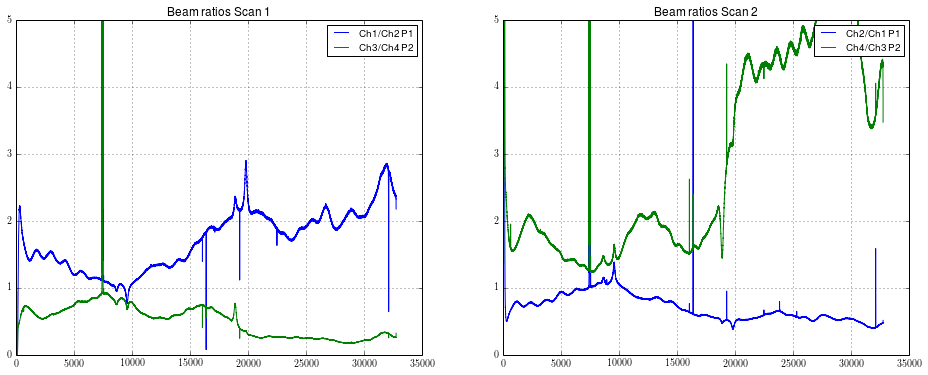
\includegraphics[max size={\textwidth}{\textheight}]{K-Band Calibration and Reduction_files/K-Band Calibration and Reduction_20_2.png}
    \par
    \end{center}
    
            \end{InvisibleVerbatim}
            
        
    
These are ratios, not differences. The baselines are similar in shape
but inverted. So at about ch.10000 the blue ratio is about 1 in both,
but at ch.20000 the ration is about 2 in the left and 0.5 in the right.
Likewise, the green curve on the right is more or less the inverse of
the green curve on the left. This is what we expect.

By the way, the strong maser feature is seen at about ch.7500 and is
positive in both ratios. All the other spiky-like things are inverted
left to right confirming that they are undesirable artifacts, such as
RFI.

The next step is to average these ratios.

    % Make sure that atleast 4 lines are below the HR
    \needspace{4\baselineskip}

    
        \vspace{6pt}
        \makebox[0.1\linewidth]{\smaller\hfill\tt\color{nbframe-in-prompt}In\hspace{4pt}{[}12{]}:\hspace{4pt}}\\*
        \vspace{-2.65\baselineskip}
        \begin{ColorVerbatim}
            \vspace{-0.7\baselineskip}
            \begin{Verbatim}[commandchars=\\\{\}]
\PY{c}{\PYZsh{} averaged after position switch}
\PY{n}{figure}\PY{p}{(}\PY{p}{)}
\PY{n}{plot}\PY{p}{(}\PY{p}{(}\PY{n}{ratioP1sc1}\PY{o}{+}\PY{n}{ratioP1sc2}\PY{p}{)}\PY{o}{/}\PY{l+m+mi}{2}\PY{p}{,} \PY{n}{label}\PY{o}{=}\PY{l+s}{\PYZdq{}}\PY{l+s}{Pol 1}\PY{l+s}{\PYZdq{}}\PY{p}{)}
\PY{n}{plot}\PY{p}{(}\PY{p}{(}\PY{n}{ratioP2sc1}\PY{o}{+}\PY{n}{ratioP2sc2}\PY{p}{)}\PY{o}{/}\PY{l+m+mi}{2}\PY{p}{,} \PY{n}{label}\PY{o}{=}\PY{l+s}{\PYZdq{}}\PY{l+s}{Pol 2}\PY{l+s}{\PYZdq{}}\PY{p}{)}
\PY{n}{ylim}\PY{p}{(}\PY{l+m+mi}{0}\PY{p}{,}\PY{l+m+mi}{70}\PY{p}{)}
\PY{n}{ylabel}\PY{p}{(}\PY{l+s}{\PYZdq{}}\PY{l+s}{On/Off Ratio}\PY{l+s}{\PYZdq{}}\PY{p}{)}
\PY{n}{legend}\PY{p}{(}\PY{p}{)}
\PY{n}{grid}\PY{p}{(}\PY{p}{)}
\PY{n}{title}\PY{p}{(}\PY{l+s}{\PYZdq{}}\PY{l+s}{Beam and position switching}\PY{l+s}{\PYZdq{}}\PY{p}{)}
\end{Verbatim}

            
                \vspace{-0.2\baselineskip}
            
        \end{ColorVerbatim}
    

    

        % If the first block is an image, minipage the image.  Else
        % request a certain amount of space for the input text.
        \needspace{4\baselineskip}
        
        

            % Add document contents.
            
                \makebox[0.1\linewidth]{\smaller\hfill\tt\color{nbframe-out-prompt}Out\hspace{4pt}{[}12{]}:\hspace{4pt}}\\*
                \vspace{-2.55\baselineskip}\begin{InvisibleVerbatim}
                \vspace{-0.5\baselineskip}
\begin{alltt}<matplotlib.text.Text at 0x7fdba7f8c1d0>\end{alltt}

            \end{InvisibleVerbatim}
            
                \begin{InvisibleVerbatim}
                \vspace{-0.5\baselineskip}
    \begin{center}
    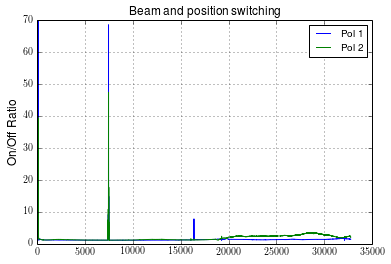
\includegraphics[max size={\textwidth}{\textheight}]{K-Band Calibration and Reduction_files/K-Band Calibration and Reduction_22_1.png}
    \par
    \end{center}
    
            \end{InvisibleVerbatim}
            
        
    
The baseline is quite flat but not perfect. Let's expand the scale.

    % Make sure that atleast 4 lines are below the HR
    \needspace{4\baselineskip}

    
        \vspace{6pt}
        \makebox[0.1\linewidth]{\smaller\hfill\tt\color{nbframe-in-prompt}In\hspace{4pt}{[}13{]}:\hspace{4pt}}\\*
        \vspace{-2.65\baselineskip}
        \begin{ColorVerbatim}
            \vspace{-0.7\baselineskip}
            \begin{Verbatim}[commandchars=\\\{\}]
\PY{n}{figure}\PY{p}{(}\PY{p}{)}
\PY{n}{plot}\PY{p}{(}\PY{p}{(}\PY{n}{ratioP1sc1}\PY{o}{+}\PY{n}{ratioP1sc2}\PY{p}{)}\PY{o}{/}\PY{l+m+mi}{2}\PY{p}{,} \PY{n}{label}\PY{o}{=}\PY{l+s}{\PYZdq{}}\PY{l+s}{Pol 1}\PY{l+s}{\PYZdq{}}\PY{p}{)}
\PY{n}{plot}\PY{p}{(}\PY{p}{(}\PY{n}{ratioP2sc1}\PY{o}{+}\PY{n}{ratioP2sc2}\PY{p}{)}\PY{o}{/}\PY{l+m+mi}{2}\PY{p}{,} \PY{n}{label}\PY{o}{=}\PY{l+s}{\PYZdq{}}\PY{l+s}{Pol 2}\PY{l+s}{\PYZdq{}}\PY{p}{)}
\PY{n}{ylim}\PY{p}{(}\PY{l+m+mi}{0}\PY{p}{,}\PY{l+m+mi}{7}\PY{p}{)}
\PY{n}{ylabel}\PY{p}{(}\PY{l+s}{\PYZdq{}}\PY{l+s}{On/Off Ratio}\PY{l+s}{\PYZdq{}}\PY{p}{)}
\PY{n}{legend}\PY{p}{(}\PY{p}{)}
\PY{n}{grid}\PY{p}{(}\PY{p}{)}
\PY{n}{title}\PY{p}{(}\PY{l+s}{\PYZdq{}}\PY{l+s}{Beam and position switching}\PY{l+s}{\PYZdq{}}\PY{p}{)}
\end{Verbatim}

            
                \vspace{-0.2\baselineskip}
            
        \end{ColorVerbatim}
    

    

        % If the first block is an image, minipage the image.  Else
        % request a certain amount of space for the input text.
        \needspace{4\baselineskip}
        
        

            % Add document contents.
            
                \makebox[0.1\linewidth]{\smaller\hfill\tt\color{nbframe-out-prompt}Out\hspace{4pt}{[}13{]}:\hspace{4pt}}\\*
                \vspace{-2.55\baselineskip}\begin{InvisibleVerbatim}
                \vspace{-0.5\baselineskip}
\begin{alltt}<matplotlib.text.Text at 0x7fdba7edf750>\end{alltt}

            \end{InvisibleVerbatim}
            
                \begin{InvisibleVerbatim}
                \vspace{-0.5\baselineskip}
    \begin{center}
    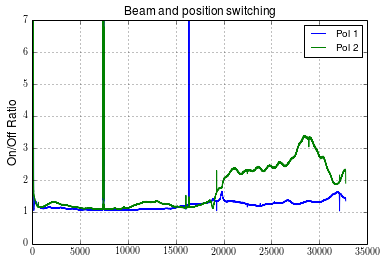
\includegraphics[max size={\textwidth}{\textheight}]{K-Band Calibration and Reduction_files/K-Band Calibration and Reduction_24_1.png}
    \par
    \end{center}
    
            \end{InvisibleVerbatim}
            
        
    
On reflection, averaging the ratio A1/A2 with the ratio A2/A1 is not
valid. It does not cancel the baseline.

$\frac{1}{2} \left ( \frac{A_1}{A_2} + \frac{A_2}{A_1} \right ) = \frac{A_1^2 - A_2^2}{2 A_1 A_2}$

\subsubsection{By Differences}\label{by-differences}

What we need to do is subtract the off from the on and then normalize by
the average of the offs.

$\frac{ \frac{1}{2} \left[ (A_1-A_2) + (A_2-A_1) \right] }  { \frac{1}{2}              (A_1+A_2)               } =     \frac{      (A_1-A_2) + (A_2-A_1)}         { \frac{1}{2} (A_1+A_2)}$

So let's give that a try.

    % Make sure that atleast 4 lines are below the HR
    \needspace{4\baselineskip}

    
        \vspace{6pt}
        \makebox[0.1\linewidth]{\smaller\hfill\tt\color{nbframe-in-prompt}In\hspace{4pt}{[}14{]}:\hspace{4pt}}\\*
        \vspace{-2.65\baselineskip}
        \begin{ColorVerbatim}
            \vspace{-0.7\baselineskip}
            \begin{Verbatim}[commandchars=\\\{\}]
\PY{c}{\PYZsh{} beam to beam ratio spectra, one for each pol}

\PY{c}{\PYZsh{} scan 1 on\PYZhy{}off}
\PY{c}{\PYZsh{} pol 1}
\PY{n}{diffP1sc1} \PY{o}{=} \PY{n}{specA1P1sc1} \PY{o}{\PYZhy{}} \PY{n}{specA2P1sc1}
\PY{c}{\PYZsh{} pol 2}
\PY{n}{diffP2sc1} \PY{o}{=} \PY{n}{specA1P2sc1} \PY{o}{\PYZhy{}} \PY{n}{specA2P2sc1}

\PY{c}{\PYZsh{} scan 2 on\PYZhy{}off}
\PY{c}{\PYZsh{} pol 1}
\PY{n}{diffP1sc2} \PY{o}{=} \PY{n}{specA2P1sc2} \PY{o}{\PYZhy{}} \PY{n}{specA1P1sc2}
\PY{c}{\PYZsh{} pol 2}
\PY{n}{diffP2sc2} \PY{o}{=} \PY{n}{specA2P2sc2} \PY{o}{\PYZhy{}} \PY{n}{specA1P2sc2}

\PY{c}{\PYZsh{} mean on\PYZhy{}off}
\PY{c}{\PYZsh{} pol 1}
\PY{n}{diffP1} \PY{o}{=} \PY{p}{(}\PY{n}{diffP1sc1}\PY{o}{+}\PY{n}{diffP1sc2}\PY{p}{)}\PY{o}{/}\PY{l+m+mi}{2}
\PY{c}{\PYZsh{} pol 2}
\PY{n}{diffP2} \PY{o}{=} \PY{p}{(}\PY{n}{diffP2sc1}\PY{o}{+}\PY{n}{diffP2sc2}\PY{p}{)}\PY{o}{/}\PY{l+m+mi}{2}

\PY{c}{\PYZsh{} mean off}
\PY{c}{\PYZsh{} pol 1}
\PY{n}{meanP1} \PY{o}{=} \PY{p}{(}\PY{n}{specA2P1sc1} \PY{o}{+} \PY{n}{specA1P1sc2}\PY{p}{)}\PY{o}{/}\PY{l+m+mi}{2}
\PY{c}{\PYZsh{} pol 2}
\PY{n}{meanP2} \PY{o}{=} \PY{p}{(}\PY{n}{specA2P2sc1} \PY{o}{+} \PY{n}{specA1P2sc2}\PY{p}{)}\PY{o}{/}\PY{l+m+mi}{2}

\PY{n}{plot}\PY{p}{(}\PY{n}{diffP1}\PY{o}{/}\PY{n}{meanP1}\PY{p}{,} \PY{n}{label}\PY{o}{=}\PY{l+s}{\PYZdq{}}\PY{l+s}{P1}\PY{l+s}{\PYZdq{}}\PY{p}{)}
\PY{n}{plot}\PY{p}{(}\PY{n}{diffP2}\PY{o}{/}\PY{n}{meanP2}\PY{p}{,} \PY{n}{label}\PY{o}{=}\PY{l+s}{\PYZdq{}}\PY{l+s}{P2}\PY{l+s}{\PYZdq{}}\PY{p}{)}
\PY{n}{title}\PY{p}{(}\PY{l+s}{\PYZdq{}}\PY{l+s}{Normalized Differences}\PY{l+s}{\PYZdq{}}\PY{p}{)}
\PY{n}{grid}\PY{p}{(}\PY{n+nb+bp}{True}\PY{p}{)}
\PY{n}{legend}\PY{p}{(}\PY{p}{)}
\end{Verbatim}

            
                \vspace{-0.2\baselineskip}
            
        \end{ColorVerbatim}
    

    

        % If the first block is an image, minipage the image.  Else
        % request a certain amount of space for the input text.
        \needspace{4\baselineskip}
        
        

            % Add document contents.
            
                \makebox[0.1\linewidth]{\smaller\hfill\tt\color{nbframe-out-prompt}Out\hspace{4pt}{[}14{]}:\hspace{4pt}}\\*
                \vspace{-2.55\baselineskip}\begin{InvisibleVerbatim}
                \vspace{-0.5\baselineskip}
\begin{alltt}<matplotlib.legend.Legend at 0x7fdba7ea8fd0>\end{alltt}

            \end{InvisibleVerbatim}
            
                \begin{InvisibleVerbatim}
                \vspace{-0.5\baselineskip}
    \begin{center}
    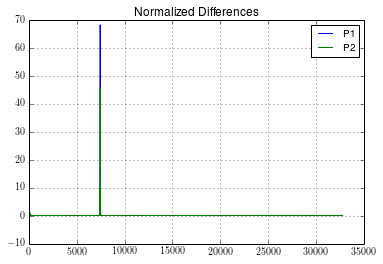
\includegraphics[max size={\textwidth}{\textheight}]{K-Band Calibration and Reduction_files/K-Band Calibration and Reduction_26_1.png}
    \par
    \end{center}
    
            \end{InvisibleVerbatim}
            
        
    
These ratio spectra can then be converted to antenna temperature by
scaling with the average off source system temperature. Now let's check
the baseline.

    % Make sure that atleast 4 lines are below the HR
    \needspace{4\baselineskip}

    
        \vspace{6pt}
        \makebox[0.1\linewidth]{\smaller\hfill\tt\color{nbframe-in-prompt}In\hspace{4pt}{[}15{]}:\hspace{4pt}}\\*
        \vspace{-2.65\baselineskip}
        \begin{ColorVerbatim}
            \vspace{-0.7\baselineskip}
            \begin{Verbatim}[commandchars=\\\{\}]
\PY{n}{plot}\PY{p}{(}\PY{n}{diffP1}\PY{o}{/}\PY{n}{meanP1}\PY{p}{,} \PY{n}{label}\PY{o}{=}\PY{l+s}{\PYZdq{}}\PY{l+s}{P1}\PY{l+s}{\PYZdq{}}\PY{p}{)}
\PY{n}{plot}\PY{p}{(}\PY{n}{diffP2}\PY{o}{/}\PY{n}{meanP2}\PY{p}{,} \PY{n}{label}\PY{o}{=}\PY{l+s}{\PYZdq{}}\PY{l+s}{P2}\PY{l+s}{\PYZdq{}}\PY{p}{)}
\PY{n}{ylim}\PY{p}{(}\PY{o}{\PYZhy{}}\PY{l+m+mf}{0.5}\PY{p}{,}\PY{l+m+mf}{0.5}\PY{p}{)}
\PY{n}{title}\PY{p}{(}\PY{l+s}{\PYZdq{}}\PY{l+s}{Normalized Differences}\PY{l+s}{\PYZdq{}}\PY{p}{)}
\PY{n}{grid}\PY{p}{(}\PY{n+nb+bp}{True}\PY{p}{)}
\PY{n}{legend}\PY{p}{(}\PY{p}{)}
\end{Verbatim}

            
                \vspace{-0.2\baselineskip}
            
        \end{ColorVerbatim}
    

    

        % If the first block is an image, minipage the image.  Else
        % request a certain amount of space for the input text.
        \needspace{4\baselineskip}
        
        

            % Add document contents.
            
                \makebox[0.1\linewidth]{\smaller\hfill\tt\color{nbframe-out-prompt}Out\hspace{4pt}{[}15{]}:\hspace{4pt}}\\*
                \vspace{-2.55\baselineskip}\begin{InvisibleVerbatim}
                \vspace{-0.5\baselineskip}
\begin{alltt}<matplotlib.legend.Legend at 0x7fdba7dfa350>\end{alltt}

            \end{InvisibleVerbatim}
            
                \begin{InvisibleVerbatim}
                \vspace{-0.5\baselineskip}
    \begin{center}
    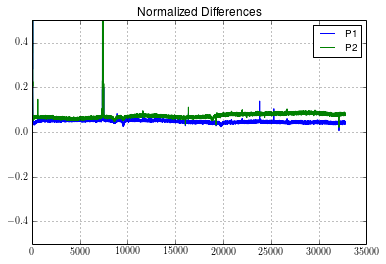
\includegraphics[max size={\textwidth}{\textheight}]{K-Band Calibration and Reduction_files/K-Band Calibration and Reduction_28_1.png}
    \par
    \end{center}
    
            \end{InvisibleVerbatim}
            
        
    
Much better! Now let's look at the line.

    % Make sure that atleast 4 lines are below the HR
    \needspace{4\baselineskip}

    
        \vspace{6pt}
        \makebox[0.1\linewidth]{\smaller\hfill\tt\color{nbframe-in-prompt}In\hspace{4pt}{[}16{]}:\hspace{4pt}}\\*
        \vspace{-2.65\baselineskip}
        \begin{ColorVerbatim}
            \vspace{-0.7\baselineskip}
            \begin{Verbatim}[commandchars=\\\{\}]
\PY{n}{plot}\PY{p}{(}\PY{n}{diffP1}\PY{o}{/}\PY{n}{meanP1}\PY{p}{,} \PY{n}{label}\PY{o}{=}\PY{l+s}{\PYZdq{}}\PY{l+s}{P1}\PY{l+s}{\PYZdq{}}\PY{p}{)}
\PY{n}{plot}\PY{p}{(}\PY{n}{diffP2}\PY{o}{/}\PY{n}{meanP2}\PY{p}{,} \PY{n}{label}\PY{o}{=}\PY{l+s}{\PYZdq{}}\PY{l+s}{P2}\PY{l+s}{\PYZdq{}}\PY{p}{)}
\PY{n}{title}\PY{p}{(}\PY{l+s}{\PYZdq{}}\PY{l+s}{Normalized Differences}\PY{l+s}{\PYZdq{}}\PY{p}{)}
\PY{n}{xlim}\PY{p}{(}\PY{l+m+mi}{7300}\PY{p}{,}\PY{l+m+mi}{7600}\PY{p}{)}
\PY{n}{grid}\PY{p}{(}\PY{n+nb+bp}{True}\PY{p}{)}
\PY{n}{legend}\PY{p}{(}\PY{p}{)}
\end{Verbatim}

            
                \vspace{-0.2\baselineskip}
            
        \end{ColorVerbatim}
    

    

        % If the first block is an image, minipage the image.  Else
        % request a certain amount of space for the input text.
        \needspace{4\baselineskip}
        
        

            % Add document contents.
            
                \makebox[0.1\linewidth]{\smaller\hfill\tt\color{nbframe-out-prompt}Out\hspace{4pt}{[}16{]}:\hspace{4pt}}\\*
                \vspace{-2.55\baselineskip}\begin{InvisibleVerbatim}
                \vspace{-0.5\baselineskip}
\begin{alltt}<matplotlib.legend.Legend at 0x7fdba7c1abd0>\end{alltt}

            \end{InvisibleVerbatim}
            
                \begin{InvisibleVerbatim}
                \vspace{-0.5\baselineskip}
    \begin{center}
    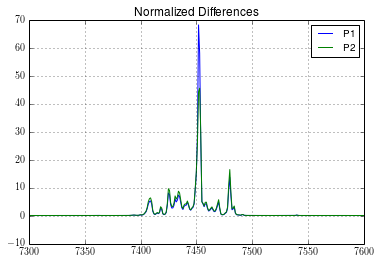
\includegraphics[max size={\textwidth}{\textheight}]{K-Band Calibration and Reduction_files/K-Band Calibration and Reduction_30_1.png}
    \par
    \end{center}
    
            \end{InvisibleVerbatim}
            
        
    
Now we scale by system temperature.

    % Make sure that atleast 4 lines are below the HR
    \needspace{4\baselineskip}

    
        \vspace{6pt}
        \makebox[0.1\linewidth]{\smaller\hfill\tt\color{nbframe-in-prompt}In\hspace{4pt}{[}17{]}:\hspace{4pt}}\\*
        \vspace{-2.65\baselineskip}
        \begin{ColorVerbatim}
            \vspace{-0.7\baselineskip}
            \begin{Verbatim}[commandchars=\\\{\}]
\PY{n}{TsysP1} \PY{o}{=} \PY{p}{(}\PY{n}{data}\PY{o}{.}\PY{n}{data}\PY{p}{[}\PY{l+s}{\PYZsq{}}\PY{l+s}{Tsys}\PY{l+s}{\PYZsq{}}\PY{p}{]}\PY{p}{[}\PY{l+m+mi}{18}\PY{p}{]}\PY{p}{[}\PY{l+m+mi}{1}\PY{p}{]}\PY{o}{+}\PY{n}{data}\PY{o}{.}\PY{n}{data}\PY{p}{[}\PY{l+s}{\PYZsq{}}\PY{l+s}{Tsys}\PY{l+s}{\PYZsq{}}\PY{p}{]}\PY{p}{[}\PY{l+m+mi}{44}\PY{p}{]}\PY{p}{[}\PY{l+m+mi}{0}\PY{p}{]}\PY{p}{)}\PY{o}{/}\PY{l+m+mi}{2}
\PY{n}{TsysP2} \PY{o}{=} \PY{p}{(}\PY{n}{data}\PY{o}{.}\PY{n}{data}\PY{p}{[}\PY{l+s}{\PYZsq{}}\PY{l+s}{Tsys}\PY{l+s}{\PYZsq{}}\PY{p}{]}\PY{p}{[}\PY{l+m+mi}{18}\PY{p}{]}\PY{p}{[}\PY{l+m+mi}{3}\PY{p}{]}\PY{o}{+}\PY{n}{data}\PY{o}{.}\PY{n}{data}\PY{p}{[}\PY{l+s}{\PYZsq{}}\PY{l+s}{Tsys}\PY{l+s}{\PYZsq{}}\PY{p}{]}\PY{p}{[}\PY{l+m+mi}{44}\PY{p}{]}\PY{p}{[}\PY{l+m+mi}{2}\PY{p}{]}\PY{p}{)}\PY{o}{/}\PY{l+m+mi}{2}
\PY{k}{print} \PY{l+s}{\PYZdq{}}\PY{l+s}{Tsys(P1)=}\PY{l+s+si}{\PYZpc{}6.1f}\PY{l+s}{K, Tsys(P2)=}\PY{l+s+si}{\PYZpc{}6.1f}\PY{l+s}{K}\PY{l+s}{\PYZdq{}} \PY{o}{\PYZpc{}} \PY{p}{(}\PY{n}{TsysP1}\PY{p}{,}\PY{n}{TsysP2}\PY{p}{)}
\PY{n}{plot}\PY{p}{(}\PY{n}{TsysP1}\PY{o}{*}\PY{n}{diffP1}\PY{o}{/}\PY{n}{meanP1}\PY{p}{,} \PY{n}{label}\PY{o}{=}\PY{l+s}{\PYZdq{}}\PY{l+s}{P1}\PY{l+s}{\PYZdq{}}\PY{p}{)}
\PY{n}{plot}\PY{p}{(}\PY{n}{TsysP2}\PY{o}{*}\PY{n}{diffP2}\PY{o}{/}\PY{n}{meanP2}\PY{p}{,} \PY{n}{label}\PY{o}{=}\PY{l+s}{\PYZdq{}}\PY{l+s}{P2}\PY{l+s}{\PYZdq{}}\PY{p}{)}
\PY{n}{title}\PY{p}{(}\PY{l+s}{\PYZdq{}}\PY{l+s}{Scaled normalized Differences}\PY{l+s}{\PYZdq{}}\PY{p}{)}
\PY{n}{xlim}\PY{p}{(}\PY{l+m+mi}{7300}\PY{p}{,}\PY{l+m+mi}{7600}\PY{p}{)}
\PY{n}{grid}\PY{p}{(}\PY{n+nb+bp}{True}\PY{p}{)}
\PY{n}{legend}\PY{p}{(}\PY{p}{)}
\end{Verbatim}

            
                \vspace{-0.2\baselineskip}
            
        \end{ColorVerbatim}
    

    

        % If the first block is an image, minipage the image.  Else
        % request a certain amount of space for the input text.
        \needspace{4\baselineskip}
        
        

            % Add document contents.
            
                \begin{InvisibleVerbatim}
                \vspace{-0.5\baselineskip}
\begin{alltt}Tsys(P1)=  67.1K, Tsys(P2)=  67.7K
\end{alltt}

            \end{InvisibleVerbatim}
            
                \makebox[0.1\linewidth]{\smaller\hfill\tt\color{nbframe-out-prompt}Out\hspace{4pt}{[}17{]}:\hspace{4pt}}\\*
                \vspace{-2.55\baselineskip}\begin{InvisibleVerbatim}
                \vspace{-0.5\baselineskip}
\begin{alltt}<matplotlib.legend.Legend at 0x7fdba7b75790>\end{alltt}

            \end{InvisibleVerbatim}
            
                \begin{InvisibleVerbatim}
                \vspace{-0.5\baselineskip}
    \begin{center}
    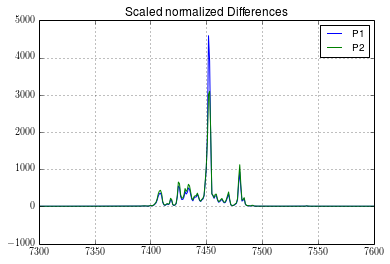
\includegraphics[max size={\textwidth}{\textheight}]{K-Band Calibration and Reduction_files/K-Band Calibration and Reduction_32_2.png}
    \par
    \end{center}
    
            \end{InvisibleVerbatim}
            
        
    
That's within the range of the other results. Off-hand I'd say the
pointing results in fluxes $\pm30$\%. It would be good to write a little
program to repeat this exercise record by record.\section{Testing Versions of
\texttt{reduce\_rrl}}\label{testing-versions-of-reduceux5frrl}

\subsection{Version Incompatibility}\label{version-incompatibility}

We need to verify the reduction done by the program
\texttt{reduce\_rrl}. The latest version which I got from Jorge is
\texttt{reduce\_rrl\_psw\_v2.0\_oldway\_quick.py} attached to an e-mail
from Jorge on 05/03/2017 04:34 PM. The various versions that exist in
\texttt{MonitorControl/BackEnds/ROACH1/apps} are

I need to see which one is used normally.

Jorge says it is the ``quick'' version. I can't compare it with
\texttt{diff} because the entire files differ. The program is simple
enough but it uses locally defined functions extracted from the class
\texttt{SAOdataset}. So I will copy the file to
\texttt{Data\_Reduction/DSN/SAO/doc} and treat it as a module.

We'll use the DOY 126 Orion KL water maser data.

    % Make sure that atleast 4 lines are below the HR
    \needspace{4\baselineskip}

    
        \vspace{6pt}
        \makebox[0.1\linewidth]{\smaller\hfill\tt\color{nbframe-in-prompt}In\hspace{4pt}{[}18{]}:\hspace{4pt}}\\*
        \vspace{-2.65\baselineskip}
        \begin{ColorVerbatim}
            \vspace{-0.7\baselineskip}
            \begin{Verbatim}[commandchars=\\\{\}]
\PY{k+kn}{from} \PY{n+nn}{reduce\PYZus{}rrl\PYZus{}psw} \PY{k+kn}{import} \PY{o}{*}

\PY{n}{average\PYZus{}spec}\PY{p}{,} \PY{n}{tau} \PY{o}{=} \PY{n}{average\PYZus{}calibrated\PYZus{}spectrum}\PY{p}{(}\PY{n}{data}\PY{p}{)}
\end{Verbatim}

            
                \vspace{-0.2\baselineskip}
            
        \end{ColorVerbatim}
    

    

        % If the first block is an image, minipage the image.  Else
        % request a certain amount of space for the input text.
        \needspace{4\baselineskip}
        
        

            % Add document contents.
            
                
            \begin{alltt}

        --------------------------------------------------------------
-------------
    AttributeError                            Traceback (most recent
call last)



        <ipython-input-18-e9de537d97ec> in <module>()
          1 from reduce\_rrl\_psw import *
          2
    ----> 3 average\_spec, tau = average\_calibrated\_spectrum(data)




        /home/local/lib/python2.7/DSN-Sci-
packages/Data\_Reduction/DSN/SAO/doc/reduce\_rrl\_psw.py in
average\_calibrated\_spectrum(self)
        138     scans = array(self.data.keys())
        139     self.logger.debug("average\_calibrated\_spectrum: for
scans \%s", scans)
    --> 140     n\_chans = self.data[1].shape[0]
        141     average\_spectra = \{0: zeros((n\_chans)), 1:
zeros((n\_chans))\}
        142     total\_records = 0




        /usr/lib/python2.7/dist-packages/h5py/\_hl/group.pyc in
\_\_getitem\_\_(self, name)
        151                 raise ValueError("Invalid HDF5 object
reference")
        152         else:
    --> 153             oid = h5o.open(self.id, self.\_e(name),
lapl=self.\_lapl)
        154
        155         otype = h5i.get\_type(oid)




        /usr/lib/python2.7/dist-packages/h5py/\_hl/base.pyc in \_e(self,
name, lcpl)
        111         else:
        112             try:
    --> 113                 name = name.encode('ascii')
        114                 coding = h5t.CSET\_ASCII
        115             except UnicodeEncodeError:




        AttributeError: 'int' object has no attribute 'encode'

\end{alltt}
        
            
        
    
This is an unexpected response. That is because the main program was not
set off with an \texttt{if \_\_name\_\_ == "\_\_main\_\_"}. Need to
change that.

    % Make sure that atleast 4 lines are below the HR
    \needspace{4\baselineskip}

    
        \vspace{6pt}
        \makebox[0.1\linewidth]{\smaller\hfill\tt\color{nbframe-in-prompt}In\hspace{4pt}{[}19{]}:\hspace{4pt}}\\*
        \vspace{-2.65\baselineskip}
        \begin{ColorVerbatim}
            \vspace{-0.7\baselineskip}
            \begin{Verbatim}[commandchars=\\\{\}]
\PY{k+kn}{from} \PY{n+nn}{reduce\PYZus{}rrl\PYZus{}psw} \PY{k+kn}{import} \PY{o}{*}

\PY{n}{average\PYZus{}spec}\PY{p}{,} \PY{n}{tau} \PY{o}{=} \PY{n}{average\PYZus{}calibrated\PYZus{}spectrum}\PY{p}{(}\PY{n}{data}\PY{p}{)}

\PY{n}{meantime} \PY{o}{=} \PY{n}{UnixTime\PYZus{}to\PYZus{}datetime}\PY{p}{(}\PY{p}{(}\PY{n}{data}\PY{o}{.}\PY{n}{header}\PY{p}{[}\PY{l+s}{\PYZsq{}}\PY{l+s}{start}\PY{l+s}{\PYZsq{}}\PY{p}{]}
                                    \PY{o}{+}\PY{n}{data}\PY{o}{.}\PY{n}{header}\PY{p}{[}\PY{l+s}{\PYZsq{}}\PY{l+s}{end}\PY{l+s}{\PYZsq{}}\PY{p}{]}\PY{p}{)}\PY{o}{/}\PY{l+m+mi}{2}\PY{p}{)}
\PY{n}{frame} \PY{o}{=} \PY{l+s}{\PYZdq{}}\PY{l+s}{RADI\PYZhy{}LSR}\PY{l+s}{\PYZdq{}}
\PY{c}{\PYZsh{}sidereal source}
\PY{n}{spl} \PY{o}{=} \PY{n+nb+bp}{None}
\PY{n}{freq}\PY{o}{=}\PY{l+m+mf}{22235.08}
\PY{n}{source}\PY{o}{=}\PY{l+s}{\PYZdq{}}\PY{l+s}{Orion KL H2O}\PY{l+s}{\PYZdq{}}
\PY{n}{x}\PY{p}{,} \PY{n}{data}\PY{o}{.}\PY{n}{header}\PY{p}{[}\PY{l+s}{\PYZsq{}}\PY{l+s}{frame}\PY{l+s}{\PYZsq{}}\PY{p}{]}\PY{p}{,} \PY{n}{data}\PY{o}{.}\PY{n}{header}\PY{p}{[}\PY{l+s}{\PYZsq{}}\PY{l+s}{velocity}\PY{l+s}{\PYZsq{}}\PY{p}{]} \PY{o}{=} \PY{n}{compute\PYZus{}X\PYZus{}axis}\PY{p}{(}\PY{n}{data}\PY{o}{.}\PY{n}{data}\PY{p}{,}
                                                         \PY{n}{frame}\PY{p}{,} \PY{l+m+mi}{43}\PY{p}{,}
                                                         \PY{n}{vspline}\PY{o}{=}\PY{n}{spl}\PY{p}{,}
                                                         \PY{n}{ref\PYZus{}freq}\PY{o}{=}\PY{n}{freq}\PY{p}{,}
                                                         \PY{n}{time}\PY{o}{=}\PY{n}{meantime}\PY{p}{)}
\PY{n}{plot}\PY{p}{(}\PY{n}{x}\PY{p}{,}\PY{n}{average\PYZus{}spec}\PY{p}{)}
\end{Verbatim}

            
                \vspace{-0.2\baselineskip}
            
        \end{ColorVerbatim}
    

    

        % If the first block is an image, minipage the image.  Else
        % request a certain amount of space for the input text.
        \needspace{4\baselineskip}
        
        

            % Add document contents.
            
                
            \begin{alltt}

        --------------------------------------------------------------
-------------
    AttributeError                            Traceback (most recent
call last)



        <ipython-input-19-d76d660b3589> in <module>()
          1 from reduce\_rrl\_psw import *
          2
    ----> 3 average\_spec, tau = average\_calibrated\_spectrum(data)
          4
          5 meantime = UnixTime\_to\_datetime((data.header['start']




        /home/local/lib/python2.7/DSN-Sci-
packages/Data\_Reduction/DSN/SAO/doc/reduce\_rrl\_psw.py in
average\_calibrated\_spectrum(self)
        138     scans = array(self.data.keys())
        139     self.logger.debug("average\_calibrated\_spectrum: for
scans \%s", scans)
    --> 140     n\_chans = self.data[1].shape[0]
        141     average\_spectra = \{0: zeros((n\_chans)), 1:
zeros((n\_chans))\}
        142     total\_records = 0




        /usr/lib/python2.7/dist-packages/h5py/\_hl/group.pyc in
\_\_getitem\_\_(self, name)
        151                 raise ValueError("Invalid HDF5 object
reference")
        152         else:
    --> 153             oid = h5o.open(self.id, self.\_e(name),
lapl=self.\_lapl)
        154
        155         otype = h5i.get\_type(oid)




        /usr/lib/python2.7/dist-packages/h5py/\_hl/base.pyc in \_e(self,
name, lcpl)
        111         else:
        112             try:
    --> 113                 name = name.encode('ascii')
        114                 coding = h5t.CSET\_ASCII
        115             except UnicodeEncodeError:




        AttributeError: 'int' object has no attribute 'encode'

\end{alltt}
        
            
        
    
It looks like \texttt{average\_calibrated\_spectrum} is using an old
format for \texttt{data}.

    % Make sure that atleast 4 lines are below the HR
    \needspace{4\baselineskip}

    
        \vspace{6pt}
        \makebox[0.1\linewidth]{\smaller\hfill\tt\color{nbframe-in-prompt}In\hspace{4pt}{[}20{]}:\hspace{4pt}}\\*
        \vspace{-2.65\baselineskip}
        \begin{ColorVerbatim}
            \vspace{-0.7\baselineskip}
            \begin{Verbatim}[commandchars=\\\{\}]
\PY{n}{data}\PY{o}{.}\PY{n}{data}\PY{o}{.}\PY{n}{keys}\PY{p}{(}\PY{p}{)}
\end{Verbatim}

            
                \vspace{-0.2\baselineskip}
            
        \end{ColorVerbatim}
    

    

        % If the first block is an image, minipage the image.  Else
        % request a certain amount of space for the input text.
        \needspace{4\baselineskip}
        
        

            % Add document contents.
            
                \makebox[0.1\linewidth]{\smaller\hfill\tt\color{nbframe-out-prompt}Out\hspace{4pt}{[}20{]}:\hspace{4pt}}\\*
                \vspace{-2.55\baselineskip}\begin{InvisibleVerbatim}
                \vspace{-0.5\baselineskip}
\begin{alltt}[u'LST',
 u'NSCANS',
 u'SITEELEV',
 u'SITELAT',
 u'SITELONG',
 u'Tsys',
 u'bandwidth',
 u'current\_azel',
 u'date\_obs',
 u'integ\_time',
 u'mode',
 u'obs\_freq',
 u'observer',
 u'offsets',
 u'onsource',
 u'pol',
 u'rest\_freq',
 u'scan\_duration',
 u'scan\_number',
 u'source\_azel',
 u'source\_long\_lat',
 u'source\_name',
 u'source\_radec',
 u'spectraCh1',
 u'spectraCh2',
 u'spectraCh3',
 u'spectraCh4',
 u'time\_obs',
 u'timestamp',
 u'v\_ref',
 u'vsys',
 u'weather']\end{alltt}

            \end{InvisibleVerbatim}
            
        
    
It looks like this is a really old version which is not compatible with
the current \texttt{SAOhdf5} class. How can I test Jorge's program then?

\subsection{Using Old Version \texttt{pickle}
File}\label{using-old-version-pickle-file}

I got a copy of the \texttt{pickle} file generated by Jorge. I will now
follow the code from Jorge's program.

    % Make sure that atleast 4 lines are below the HR
    \needspace{4\baselineskip}

    
        \vspace{6pt}
        \makebox[0.1\linewidth]{\smaller\hfill\tt\color{nbframe-in-prompt}In\hspace{4pt}{[}21{]}:\hspace{4pt}}\\*
        \vspace{-2.65\baselineskip}
        \begin{ColorVerbatim}
            \vspace{-0.7\baselineskip}
            \begin{Verbatim}[commandchars=\\\{\}]
\PY{k+kn}{import} \PY{n+nn}{dill} \PY{k+kn}{as} \PY{n+nn}{cPickle}
\PY{n}{filename} \PY{o}{=} \PY{l+s}{\PYZdq{}}\PY{l+s}{/usr/local/project\PYZus{}data/ISM\PYZus{}RRL/dss43/2017/126/A2LiP1I1494057349.22.Orion\PYZhy{}KL.spec.pkl}\PY{l+s}{\PYZdq{}}
\PY{n}{fd} \PY{o}{=} \PY{n+nb}{open}\PY{p}{(}\PY{n}{filename}\PY{p}{,} \PY{l+s}{\PYZdq{}}\PY{l+s}{rb}\PY{l+s}{\PYZdq{}}\PY{p}{)}
\PY{n}{data} \PY{o}{=} \PY{n}{cPickle}\PY{o}{.}\PY{n}{load}\PY{p}{(}\PY{n}{fd}\PY{p}{)}
\PY{n}{fd}\PY{o}{.}\PY{n}{close}\PY{p}{(}\PY{p}{)} 
\end{Verbatim}

            
                \vspace{-0.2\baselineskip}
            
        \end{ColorVerbatim}
    


    % Make sure that atleast 4 lines are below the HR
    \needspace{4\baselineskip}

    
        \vspace{6pt}
        \makebox[0.1\linewidth]{\smaller\hfill\tt\color{nbframe-in-prompt}In\hspace{4pt}{[}22{]}:\hspace{4pt}}\\*
        \vspace{-2.65\baselineskip}
        \begin{ColorVerbatim}
            \vspace{-0.7\baselineskip}
            \begin{Verbatim}[commandchars=\\\{\}]
\PY{k+kn}{from} \PY{n+nn}{reduce\PYZus{}rrl\PYZus{}psw} \PY{k+kn}{import} \PY{o}{*}
\PY{n}{average\PYZus{}spec}\PY{p}{,} \PY{n}{tau} \PY{o}{=} \PY{n}{average\PYZus{}calibrated\PYZus{}spectrum}\PY{p}{(}\PY{n}{data}\PY{p}{)}
\PY{n}{meantime} \PY{o}{=} \PY{n}{UnixTime\PYZus{}to\PYZus{}datetime}\PY{p}{(}\PY{p}{(}\PY{n}{data}\PY{o}{.}\PY{n}{header}\PY{p}{[}\PY{l+s}{\PYZsq{}}\PY{l+s}{start}\PY{l+s}{\PYZsq{}}\PY{p}{]}
                                    \PY{o}{+}\PY{n}{data}\PY{o}{.}\PY{n}{header}\PY{p}{[}\PY{l+s}{\PYZsq{}}\PY{l+s}{end}\PY{l+s}{\PYZsq{}}\PY{p}{]}\PY{p}{)}\PY{o}{/}\PY{l+m+mi}{2}\PY{p}{)}
\PY{n}{frame} \PY{o}{=} \PY{l+s}{\PYZdq{}}\PY{l+s}{RADI\PYZhy{}LSR}\PY{l+s}{\PYZdq{}}
\PY{c}{\PYZsh{}sidereal source}
\PY{n}{spl} \PY{o}{=} \PY{n+nb+bp}{None}
\PY{n}{freq}\PY{o}{=}\PY{l+m+mf}{22235.08}
\PY{n}{source}\PY{o}{=}\PY{l+s}{\PYZdq{}}\PY{l+s}{Orion KL H2O}\PY{l+s}{\PYZdq{}}
\PY{n}{x}\PY{p}{,} \PY{n}{data}\PY{o}{.}\PY{n}{header}\PY{p}{[}\PY{l+s}{\PYZsq{}}\PY{l+s}{frame}\PY{l+s}{\PYZsq{}}\PY{p}{]}\PY{p}{,} \PY{n}{data}\PY{o}{.}\PY{n}{header}\PY{p}{[}\PY{l+s}{\PYZsq{}}\PY{l+s}{velocity}\PY{l+s}{\PYZsq{}}\PY{p}{]} \PY{o}{=} \PY{n}{compute\PYZus{}X\PYZus{}axis}\PY{p}{(}\PY{n}{data}\PY{p}{,}
                                                         \PY{n}{frame}\PY{p}{,} \PY{l+m+mi}{43}\PY{p}{,}
                                                         \PY{n}{vspline}\PY{o}{=}\PY{n}{spl}\PY{p}{,}
                                                         \PY{n}{ref\PYZus{}freq}\PY{o}{=}\PY{n}{freq}\PY{p}{,}
                                                         \PY{n}{time}\PY{o}{=}\PY{n}{meantime}\PY{p}{)}
\PY{n}{plot}\PY{p}{(}\PY{n}{average\PYZus{}spec}\PY{p}{[}\PY{l+m+mi}{0}\PY{p}{]}\PY{p}{,} \PY{n}{label}\PY{o}{=}\PY{l+s}{\PYZdq{}}\PY{l+s}{Pol 1}\PY{l+s}{\PYZdq{}}\PY{p}{)}
\PY{n}{plot}\PY{p}{(}\PY{n}{average\PYZus{}spec}\PY{p}{[}\PY{l+m+mi}{1}\PY{p}{]}\PY{p}{,} \PY{n}{label}\PY{o}{=}\PY{l+s}{\PYZdq{}}\PY{l+s}{Pol 2}\PY{l+s}{\PYZdq{}}\PY{p}{)}
\PY{n}{xlim}\PY{p}{(}\PY{l+m+mi}{7300}\PY{p}{,}\PY{l+m+mi}{7600}\PY{p}{)}
\PY{n}{grid}\PY{p}{(}\PY{n+nb+bp}{True}\PY{p}{)}
\PY{n}{legend}\PY{p}{(}\PY{p}{)}
\PY{n}{title}\PY{p}{(}\PY{l+s}{\PYZdq{}}\PY{l+s}{Average calibrated spectrum}\PY{l+s}{\PYZdq{}}\PY{p}{)}
\end{Verbatim}

            
                \vspace{-0.2\baselineskip}
            
        \end{ColorVerbatim}
    

    

        % If the first block is an image, minipage the image.  Else
        % request a certain amount of space for the input text.
        \needspace{4\baselineskip}
        
        

            % Add document contents.
            
                \begin{InvisibleVerbatim}
                \vspace{-0.5\baselineskip}
\begin{alltt}reduce\_rrl\_psw.py:197: RuntimeWarning: divide by zero encountered in
divide
  ratio1 = on1data/off2data
reduce\_rrl\_psw.py:197: RuntimeWarning: invalid value encountered in
divide
  ratio1 = on1data/off2data
\end{alltt}

            \end{InvisibleVerbatim}
            
                \makebox[0.1\linewidth]{\smaller\hfill\tt\color{nbframe-out-prompt}Out\hspace{4pt}{[}22{]}:\hspace{4pt}}\\*
                \vspace{-2.55\baselineskip}\begin{InvisibleVerbatim}
                \vspace{-0.5\baselineskip}
\begin{alltt}<matplotlib.text.Text at 0x7fdb9b51cf90>\end{alltt}

            \end{InvisibleVerbatim}
            
                \begin{InvisibleVerbatim}
                \vspace{-0.5\baselineskip}
    \begin{center}
    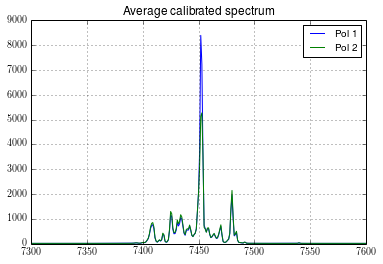
\includegraphics[max size={\textwidth}{\textheight}]{K-Band Calibration and Reduction_files/K-Band Calibration and Reduction_42_2.png}
    \par
    \end{center}
    
            \end{InvisibleVerbatim}
            
        
    
Comparing this to the plot named ``Scaled normalized differences'' we
see that this Y-scale is twice that of the previous. So we need to look
at the code for \texttt{average\_calibrated\_spectrum()} to see why.

It turns out that \texttt{average\_calibrated\_spectrum()} computes the
beam and position switched spectrum. That is what is done in
\texttt{reduce\_rrl\_psw\_v2.0\_oldway\_quick\_Kband2.py} but is not
what is done in the other versions of \texttt{reduce\_rrl\_psw}. Also,
\texttt{average\_calibrated\_spectrum()} appears to add the
beam-switched spectra instead of averaging them, which explains the
scaling problem. Now let's do it the way it is really done.

\subsection{Position Switched Reduction in
\texttt{reduce\_rrl\_psw}}\label{position-switched-reduction-in-reduceux5frrlux5fpsw}

    % Make sure that atleast 4 lines are below the HR
    \needspace{4\baselineskip}

    
        \vspace{6pt}
        \makebox[0.1\linewidth]{\smaller\hfill\tt\color{nbframe-in-prompt}In\hspace{4pt}{[}27{]}:\hspace{4pt}}\\*
        \vspace{-2.65\baselineskip}
        \begin{ColorVerbatim}
            \vspace{-0.7\baselineskip}
            \begin{Verbatim}[commandchars=\\\{\}]
\PY{n}{feed}\PY{o}{=}\PY{l+m+mi}{0}
\PY{n}{scans} \PY{o}{=} \PY{n}{data}\PY{o}{.}\PY{n}{data}\PY{o}{.}\PY{n}{keys}\PY{p}{(}\PY{p}{)}
\PY{n}{data2}\PY{o}{=}\PY{p}{[}\PY{p}{]} \PY{c}{\PYZsh{} This structure will contain all on\PYZhy{}off pairs (averaged in polarization) }

\PY{c}{\PYZsh{} Create a data structure for each scan that is all pairs of on\PYZhy{}off records.}
\PY{k}{for} \PY{n}{scan} \PY{o+ow}{in} \PY{n+nb}{range}\PY{p}{(}\PY{l+m+mi}{1}\PY{p}{,}\PY{n+nb}{len}\PY{p}{(}\PY{n}{scans}\PY{p}{)}\PY{p}{,}\PY{l+m+mi}{2}\PY{p}{)}\PY{p}{:}
    \PY{n}{onsource}\PY{o}{=}\PY{n}{data}\PY{o}{.}\PY{n}{data}\PY{p}{[}\PY{n}{scan}\PY{p}{]}\PY{p}{[}\PY{p}{:}\PY{p}{,}\PY{l+m+mi}{0}\PY{p}{,}\PY{l+m+mi}{0}\PY{p}{,}\PY{p}{:}\PY{p}{,}\PY{p}{:}\PY{p}{,}\PY{n}{feed}\PY{p}{]}
    \PY{n}{offsource}\PY{o}{=}\PY{n}{data}\PY{o}{.}\PY{n}{data}\PY{p}{[}\PY{n}{scan}\PY{o}{+}\PY{l+m+mi}{1}\PY{p}{]}\PY{p}{[}\PY{p}{:}\PY{p}{,}\PY{l+m+mi}{0}\PY{p}{,}\PY{l+m+mi}{0}\PY{p}{,}\PY{p}{:}\PY{p}{,}\PY{p}{:}\PY{p}{,}\PY{n}{feed}\PY{p}{]}

    \PY{n}{tsys}\PY{o}{=}\PY{n}{data}\PY{o}{.}\PY{n}{header}\PY{p}{[}\PY{l+s}{\PYZsq{}}\PY{l+s}{TSYS}\PY{l+s}{\PYZsq{}}\PY{p}{]}\PY{p}{[}\PY{n}{scan}\PY{p}{]}\PY{p}{[}\PY{p}{:}\PY{p}{,}\PY{p}{:}\PY{p}{,}\PY{n}{feed}\PY{p}{]}
    \PY{n}{tsys\PYZus{}ave}\PY{o}{=}\PY{n}{tsys}\PY{o}{.}\PY{n}{mean}\PY{p}{(}\PY{n}{axis}\PY{o}{=}\PY{l+m+mi}{1}\PY{p}{)}     
 
    \PY{n}{onsource\PYZus{}mean}\PY{o}{=}\PY{n}{onsource}\PY{o}{.}\PY{n}{mean}\PY{p}{(}\PY{n}{axis}\PY{o}{=}\PY{l+m+mi}{2}\PY{p}{)}
    \PY{n}{offsource\PYZus{}mean}\PY{o}{=}\PY{n}{offsource}\PY{o}{.}\PY{n}{mean}\PY{p}{(}\PY{n}{axis}\PY{o}{=}\PY{l+m+mi}{2}\PY{p}{)}
     
    \PY{n}{sdiff}\PY{o}{=}\PY{n}{ma}\PY{o}{.}\PY{n}{masked\PYZus{}invalid}\PY{p}{(}\PY{p}{(}\PY{n}{onsource\PYZus{}mean}\PY{o}{\PYZhy{}}\PY{n}{offsource\PYZus{}mean}\PY{p}{)}\PY{o}{*}\PY{p}{(}\PY{n}{tsys\PYZus{}ave}\PY{o}{/}\PY{n}{offsource\PYZus{}mean}\PY{p}{)}\PY{p}{)}
 
    \PY{n}{sdiff\PYZus{}avg}\PY{o}{=}\PY{n}{sdiff}\PY{o}{.}\PY{n}{mean}\PY{p}{(}\PY{n}{axis}\PY{o}{=}\PY{l+m+mi}{1}\PY{p}{)} \PY{c}{\PYZsh{} Polarization average}
    \PY{n}{data2}\PY{o}{.}\PY{n}{append}\PY{p}{(}\PY{n}{sdiff\PYZus{}avg}\PY{p}{)}

\PY{n}{average\PYZus{}spec}\PY{o}{=}\PY{n}{mean}\PY{p}{(}\PY{n}{data2}\PY{p}{[}\PY{p}{:}\PY{p}{]}\PY{p}{,}\PY{n}{axis}\PY{o}{=}\PY{l+m+mi}{0}\PY{p}{)} \PY{c}{\PYZsh{}Average between scans}
\PY{n}{plot}\PY{p}{(}\PY{n}{x}\PY{p}{,}\PY{n}{average\PYZus{}spec}\PY{p}{)}
\PY{n}{xlim}\PY{p}{(}\PY{o}{\PYZhy{}}\PY{l+m+mi}{100}\PY{p}{,}\PY{l+m+mi}{100}\PY{p}{)}
\PY{n}{grid}\PY{p}{(}\PY{p}{)}
\PY{n}{title}\PY{p}{(}\PY{l+s}{\PYZdq{}}\PY{l+s}{Position Switched}\PY{l+s}{\PYZdq{}}\PY{p}{)}
\end{Verbatim}

            
                \vspace{-0.2\baselineskip}
            
        \end{ColorVerbatim}
    

    

        % If the first block is an image, minipage the image.  Else
        % request a certain amount of space for the input text.
        \needspace{4\baselineskip}
        
        

            % Add document contents.
            
                \makebox[0.1\linewidth]{\smaller\hfill\tt\color{nbframe-out-prompt}Out\hspace{4pt}{[}27{]}:\hspace{4pt}}\\*
                \vspace{-2.55\baselineskip}\begin{InvisibleVerbatim}
                \vspace{-0.5\baselineskip}
\begin{alltt}<matplotlib.text.Text at 0x7fdbb3ed2890>\end{alltt}

            \end{InvisibleVerbatim}
            
                \begin{InvisibleVerbatim}
                \vspace{-0.5\baselineskip}
    \begin{center}
    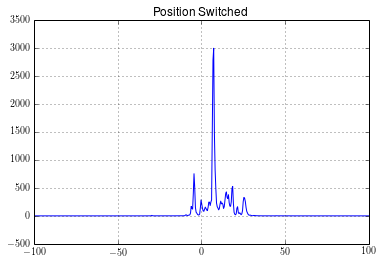
\includegraphics[max size={\textwidth}{\textheight}]{K-Band Calibration and Reduction_files/K-Band Calibration and Reduction_44_1.png}
    \par
    \end{center}
    
            \end{InvisibleVerbatim}
            
        
    
So this is a result consistent with the others.
        

        \renewcommand{\indexname}{Index}
        \printindex

    % End of document
    \end{document}


